\chapter{Исследования}

\section{Исследование первичного поля}

Пусть источник индукционного поля лежит на расстоянии $R = 500$ м от оси симметрии и имееет силу тока, равную $J_{\varphi} = 1.0$ А. Также условимся, что источник работал достаточно долго, чтобы создать стабильное электромагнитное поле. Сетка по времени равномерная: $t=[1.0; 1.05]$ на 200 временных слоёв. После истечения первой секунды мы отключим наш источник, т.е. $J_{\varphi} = 0.0$ A при $t > 1.0$. На рисунках \ref{fig:A_phi_0} -- \ref{fig:E_phi_2} представлено распространение этого поля в среде в начальный, промежуточных и последний момент времени.

\begin{figure}
	\centering
	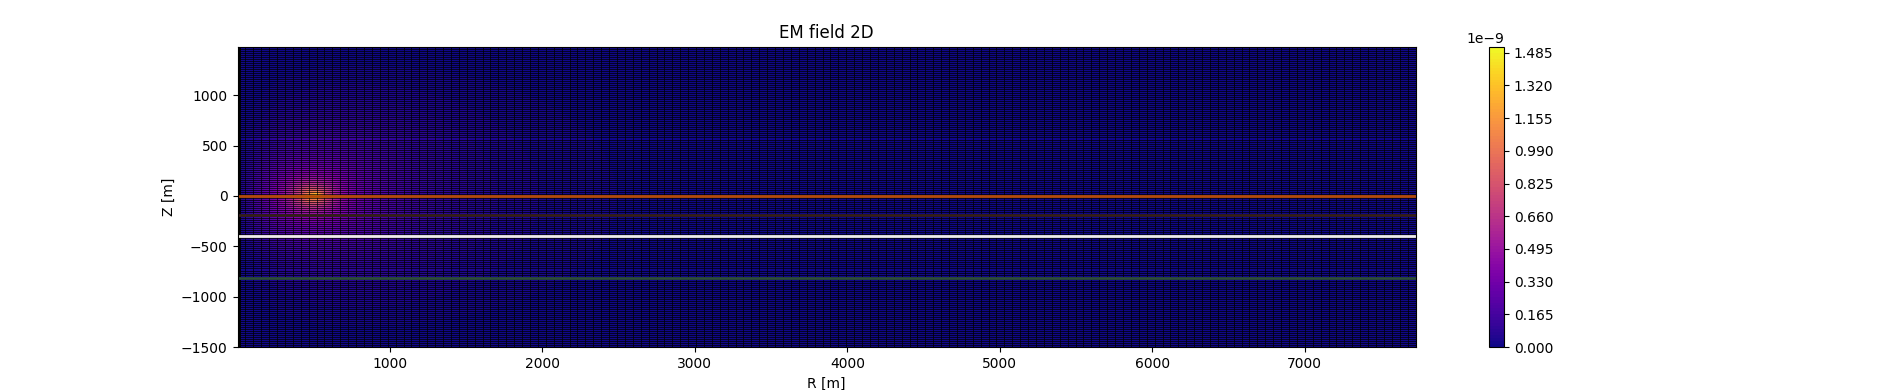
\includegraphics[width=1.0\linewidth]{images/Answer_A_time_layer_1.png}
	\caption{Решение $A_{\varphi}$ при $t = 1.0с$}
	\label{fig:A_phi_0}
\end{figure}

\begin{figure}
	\centering
	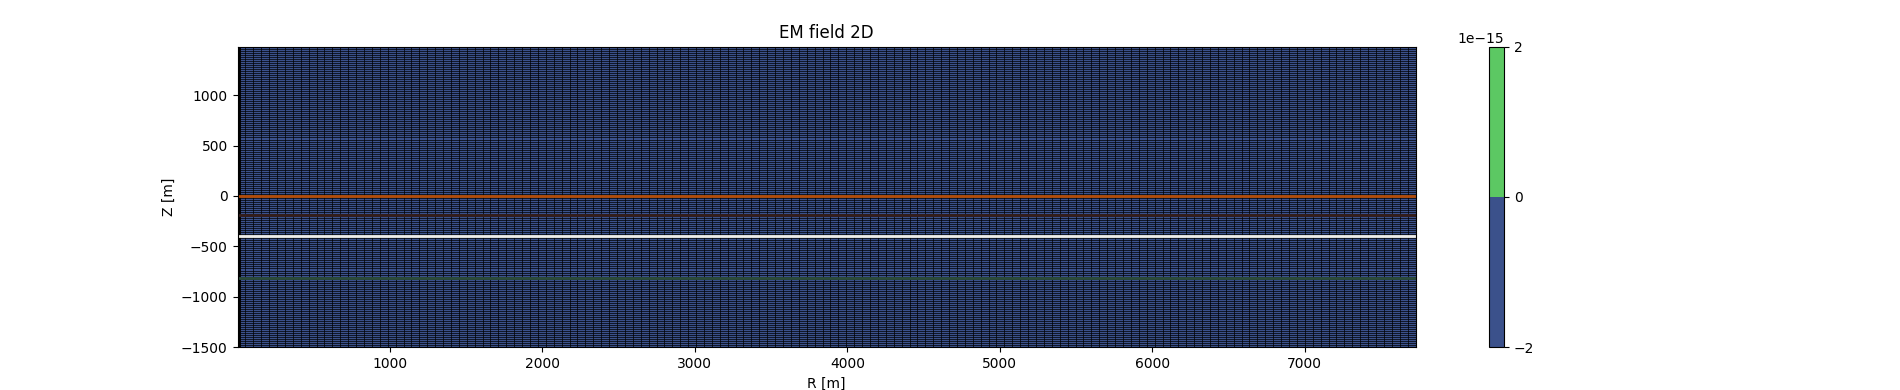
\includegraphics[width=1.0\linewidth]{images/Answer_E_time_layer_1.png}
	\caption{Решение $E_{\varphi}$ при $t = 1.0с$}
	\label{fig:E_phi_0}
\end{figure}

\begin{figure}
	\centering
	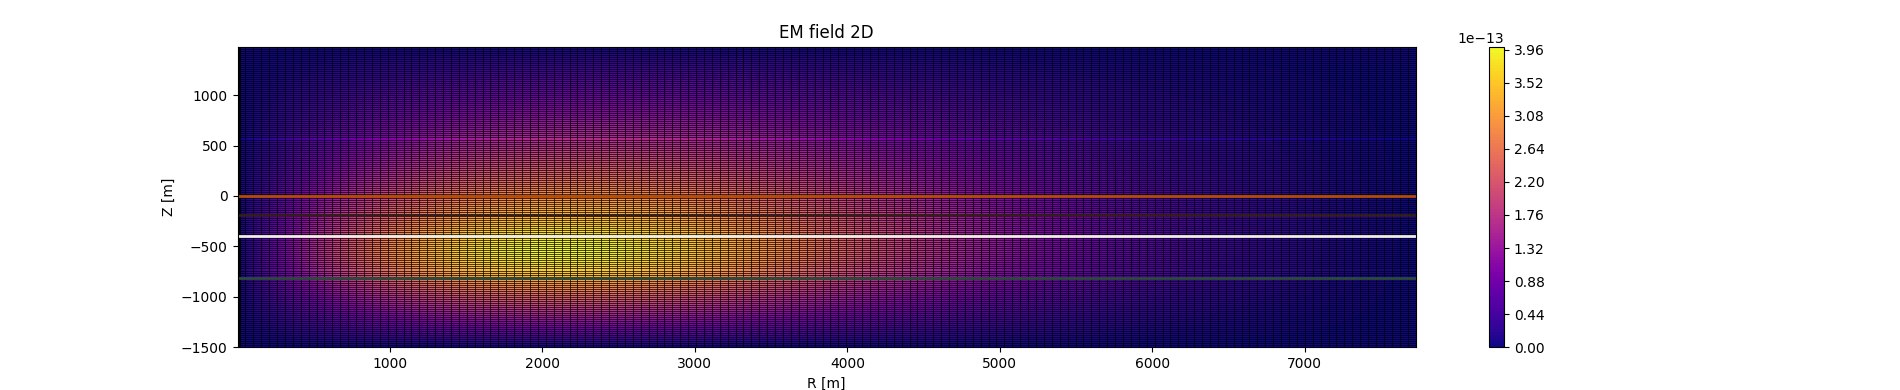
\includegraphics[width=1.0\linewidth]{images/Answer_A_time_layer_1.0250000000000083.png}
	\caption{Решение $A_{\varphi}$ при $t = 1.025с$}
	\label{fig:A_phi_1}
\end{figure}

\begin{figure}
	\centering
	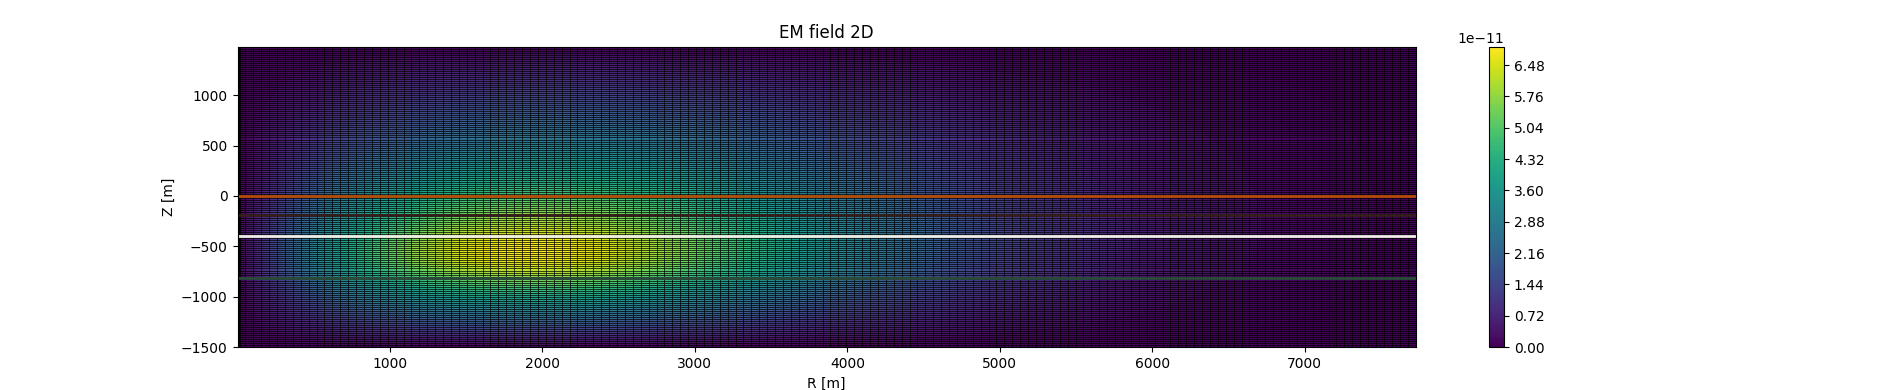
\includegraphics[width=1.0\linewidth]{images/Answer_E_time_layer_1.0250000000000083.png}
	\caption{Решение $E_{\varphi}$ при $t = 1.025с$}
	\label{fig:E_phi_1}
\end{figure} 

\begin{figure}
	\centering
	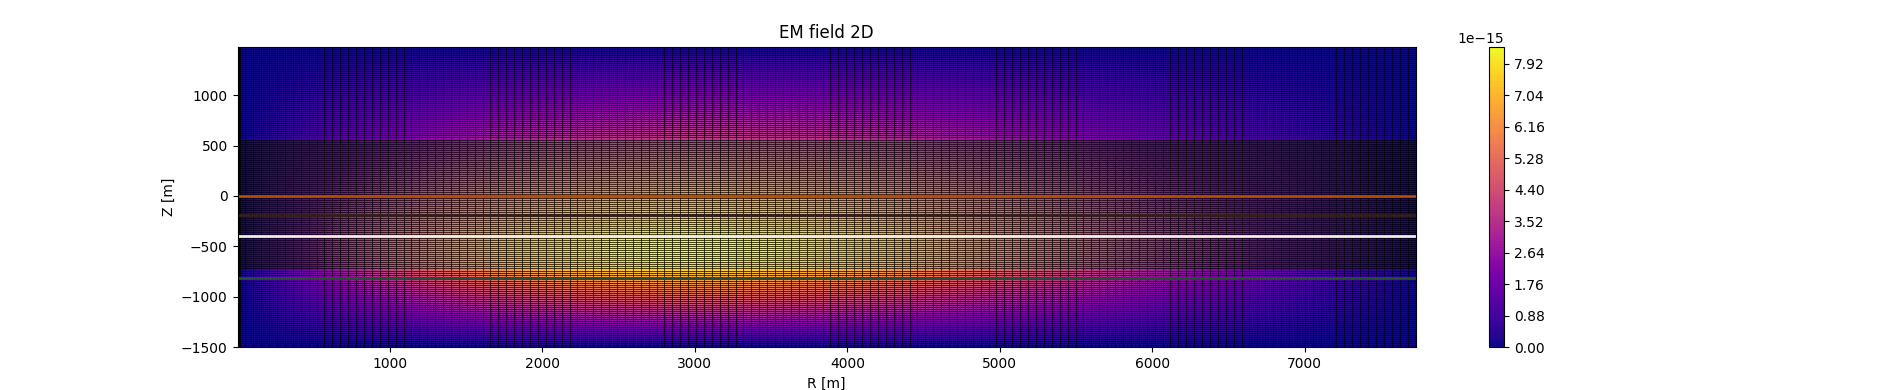
\includegraphics[width=1.0\linewidth]{images/Answer_A_time_layer_1.05.png}
	\caption{Решение $A_{\varphi}$ при $t = 1.05с$}
	\label{fig:A_phi_2}
\end{figure}

\begin{figure}
	\centering
	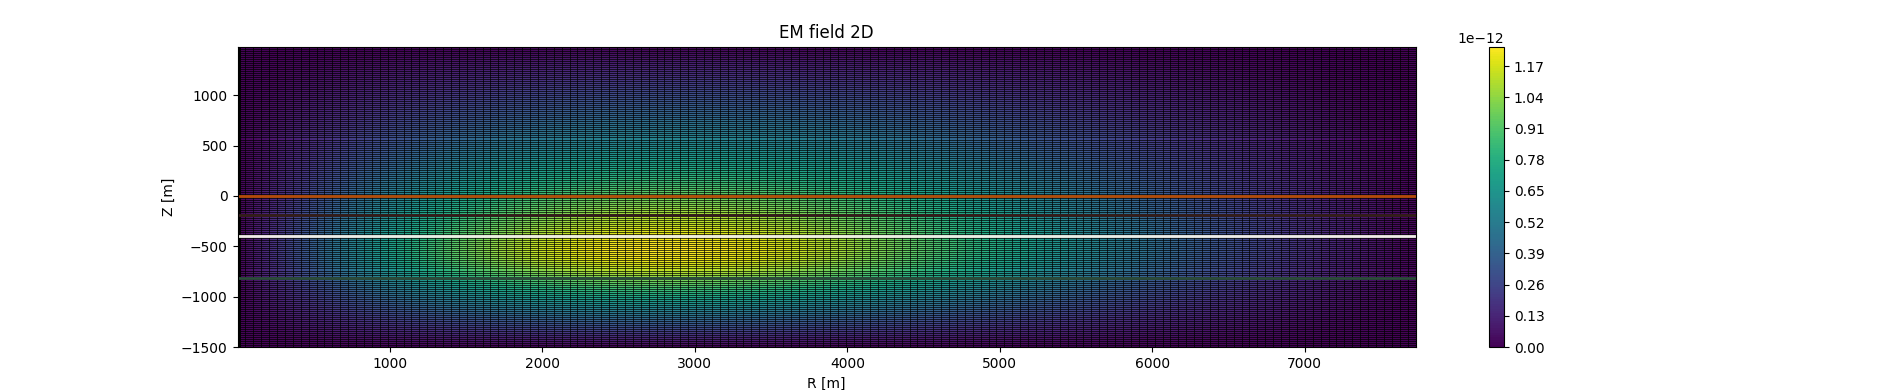
\includegraphics[width=1.0\linewidth]{images/Answer_E_time_layer_1.05.png}
	\caption{Решение $A_{\varphi}$ при $t = 1.05с$}
	\label{fig:E_phi_2}
\end{figure} 

Расположим на расчётной области приёмники в каждой горизонтально-слоистой среде и проведем замеры значений вектор-потенциала и электрического поля в точках $(2500; 0; -100)$, $(2500; 0; -200)$, $(10; 0; -700)$, $(1000; 0; -1250)$. Отобразим на графиках \ref{fig:NatA} -- \ref{fig:LogE} полученные значения.

\begin{figure}
	\centering
	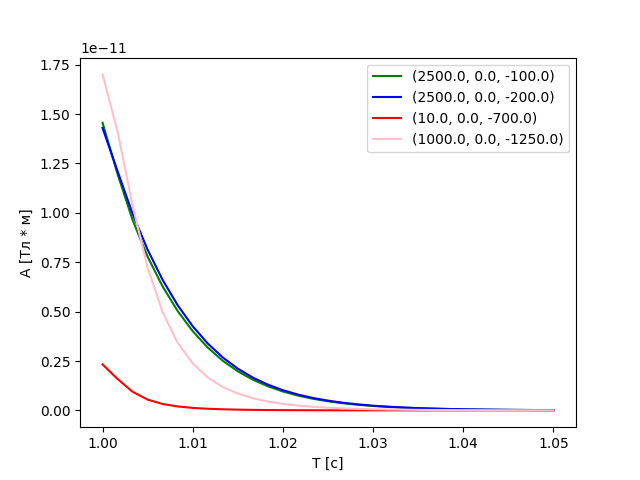
\includegraphics[width=0.8\linewidth]{images/Normal_A.png}
	\caption{Зависимость значения $A_{\varphi}$ от времени в разных приёмниках}
	\label{fig:NatA}
\end{figure}

\begin{figure}
	\centering
	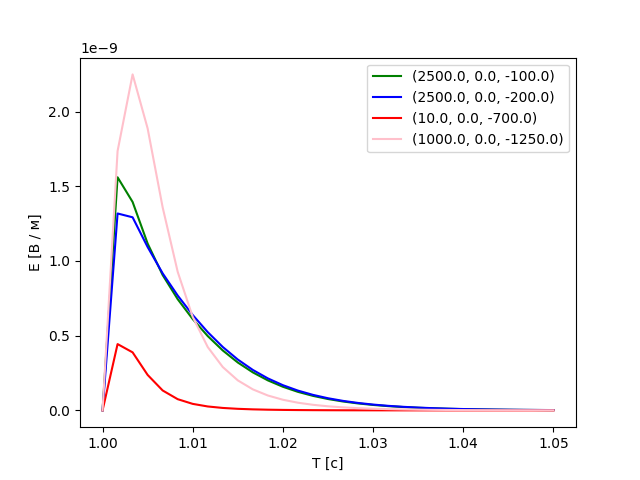
\includegraphics[width=0.8\linewidth]{images/Normal_E.png}
	\caption{Зависимость значения $E_{\varphi}$ от времени в разных приёмниках}
	\label{fig:NatE}
\end{figure}


\begin{figure}
	\centering
	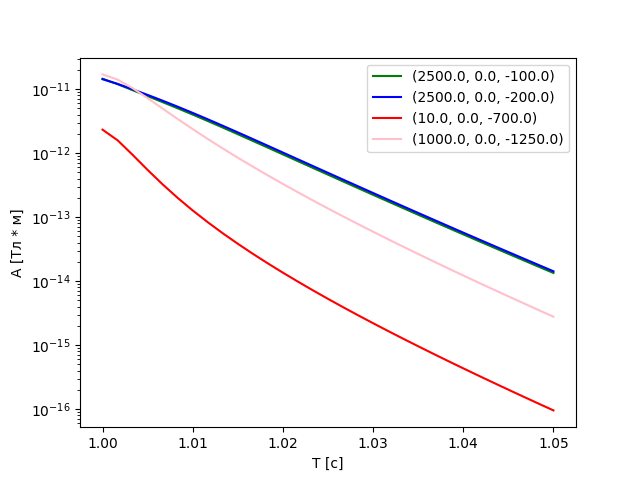
\includegraphics[width=0.8\linewidth]{images/Log_A.png}
	\caption{Зависимость значения $A_{\varphi}$ от времени в разных приёмниках (логарифмическая шкала по оси абсцисс)}
	\label{fig:LogA}
\end{figure}

\begin{figure}
	\centering
	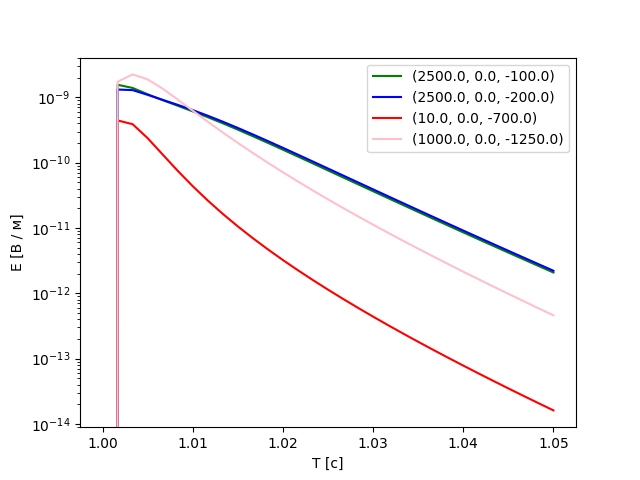
\includegraphics[width=0.8\linewidth]{images/Log_E.png}
	\caption{Зависимость значения $E_{\varphi}$ от времени в разных приёмниках (логарифмическая шкала по оси абсцисс)}
	\label{fig:LogE}
\end{figure} 

Как видим, значения вектор-потенциала и электрической напряжённости поля не имеют каких-либо резких колебаний. Из этого можно заключить, что, как и предполагалось, никаких аномальных зон в исследуемой области нет. 

\section{Исследование при разделении нормального и добавочного поля}

Добавим в нашу область аномальный объект со следующими границами: $[-5500; 5500]_x \times [2205; 2355]_y \times [-180; -80]_z$ и значением $\sigma = 4$. Будем искать решение из уравнения на добавочное поле (\ref{eq_1_6}). Получим решения изображенные на рисунках \ref{fig:A_plus_t0} -- \ref{fig:E_plus_t2}.

\begin{figure}
	\centering
	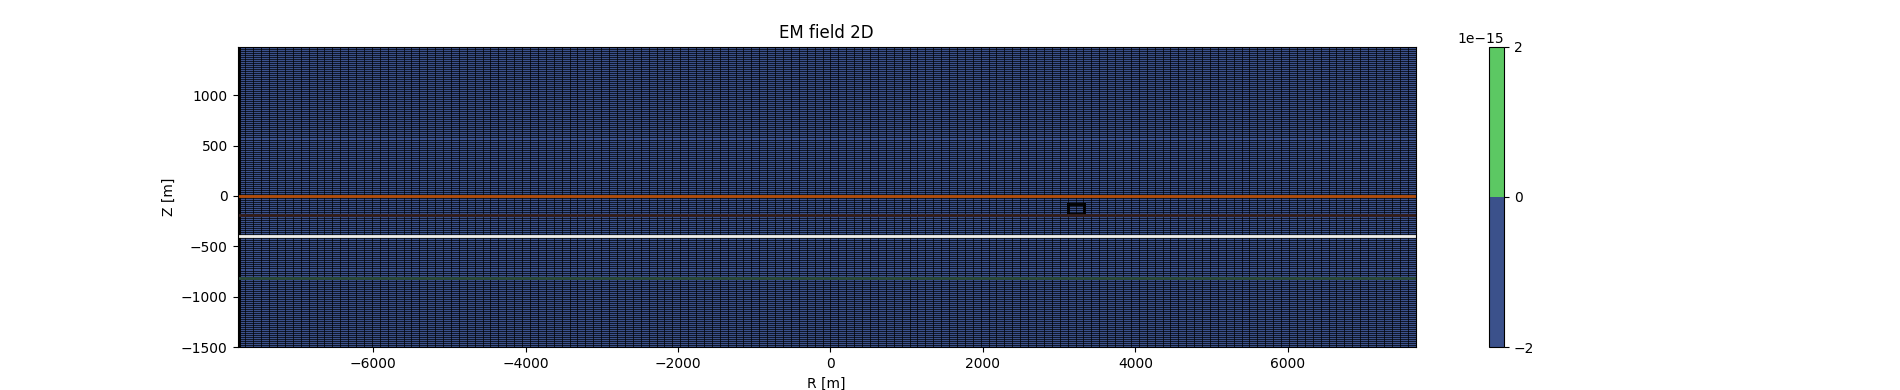
\includegraphics[width=1.0\linewidth]{images/Answer_A_plus_time_layer_1.png}
	\caption{Решение $\overrightarrow{\textbf{A}}^+$ при $t = 1.0с$}
	\label{fig:A_plus_t0}
\end{figure} 


\begin{figure}
	\centering
	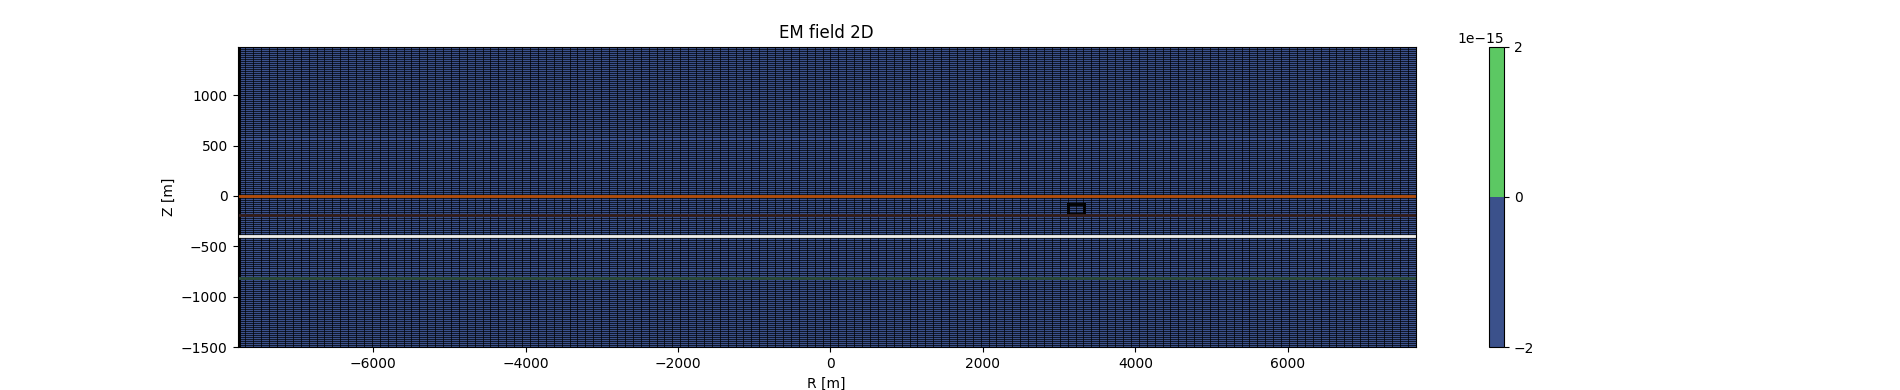
\includegraphics[width=1.0\linewidth]{images/Answer_E_plus_time_layer_1.png}
	\caption{Решение $\overrightarrow{\textbf{E}}^+$ при $t = 1.0с$}
	\label{fig:E_plus_t0}
\end{figure} 


\begin{figure}
	\centering
	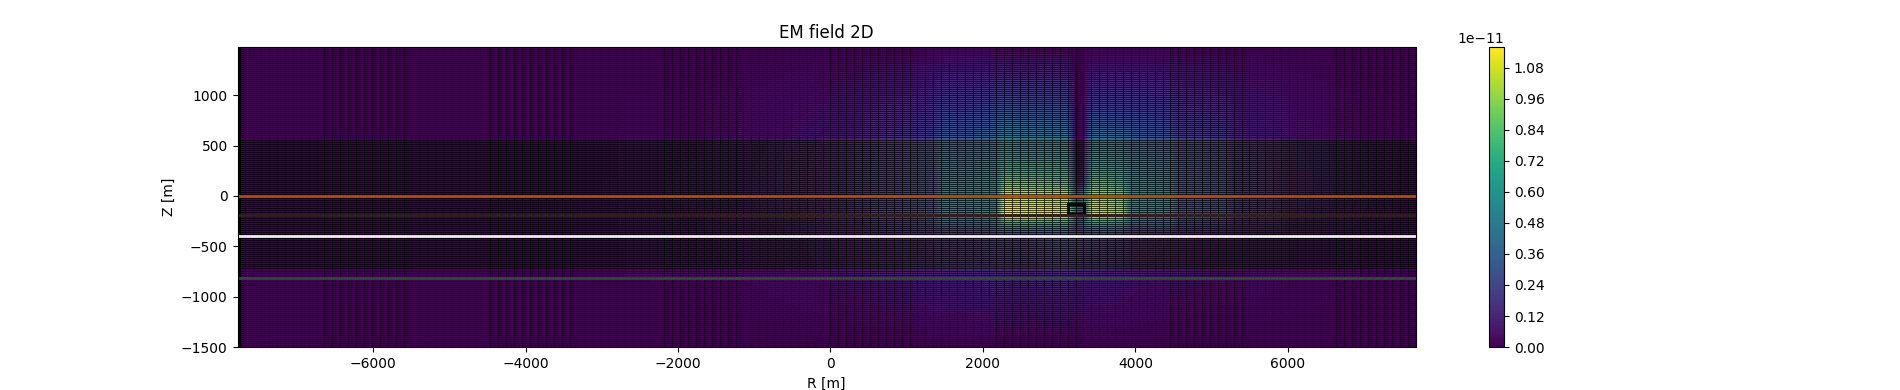
\includegraphics[width=1.0\linewidth]{images/Answer_A_plus_time_layer_1.0250000000000006.png}
	\caption{Решение $\overrightarrow{\textbf{A}}^+$ при $t = 1.025с$}
	\label{fig:A_plus_t1}
\end{figure} 


\begin{figure}
	\centering
	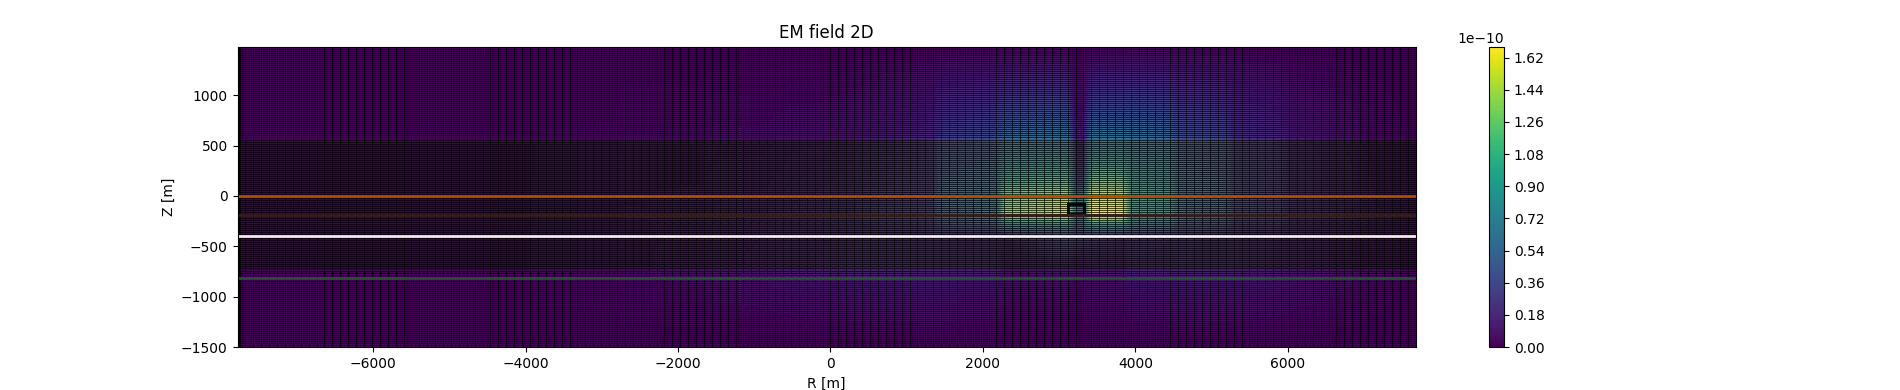
\includegraphics[width=1.0\linewidth]{images/Answer_E_plus_time_layer_1.0250000000000006.png}
	\caption{Решение $\overrightarrow{\textbf{E}}^+$ при $t = 1.025с$}
	\label{fig:E_plus_t1}
\end{figure} 

\begin{figure}
	\centering
	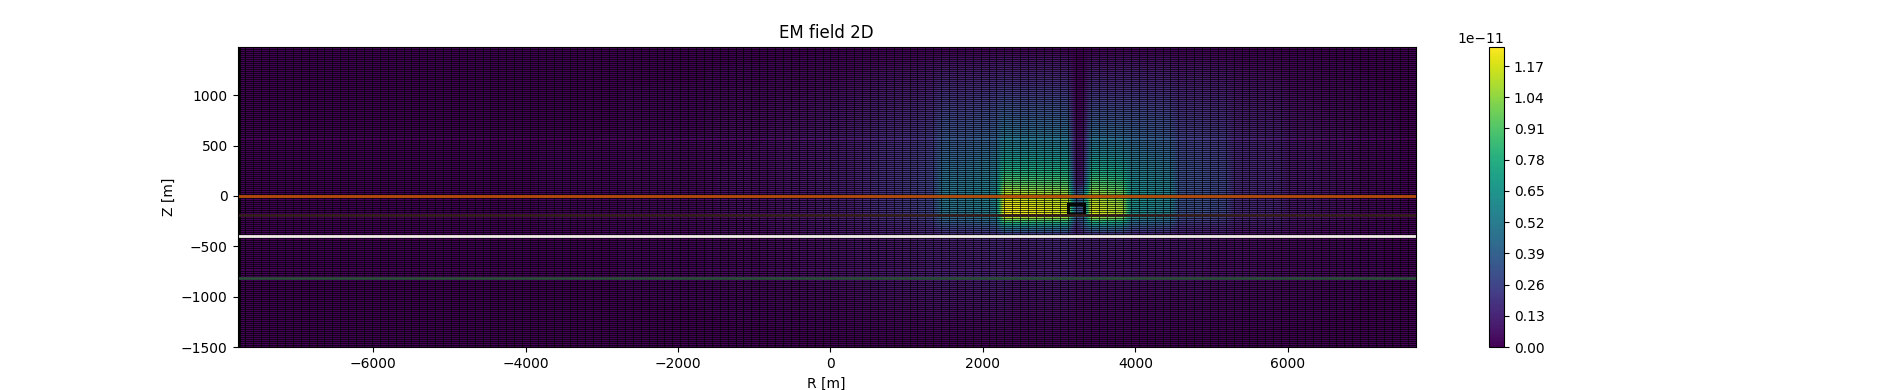
\includegraphics[width=1.0\linewidth]{images/Answer_A_plus_time_layer_1.05.png}
	\caption{Решение $\overrightarrow{\textbf{A}}^+$ при $t = 1.05с$}
	\label{fig:A_plus_t2}
\end{figure} 


\begin{figure}
	\centering
	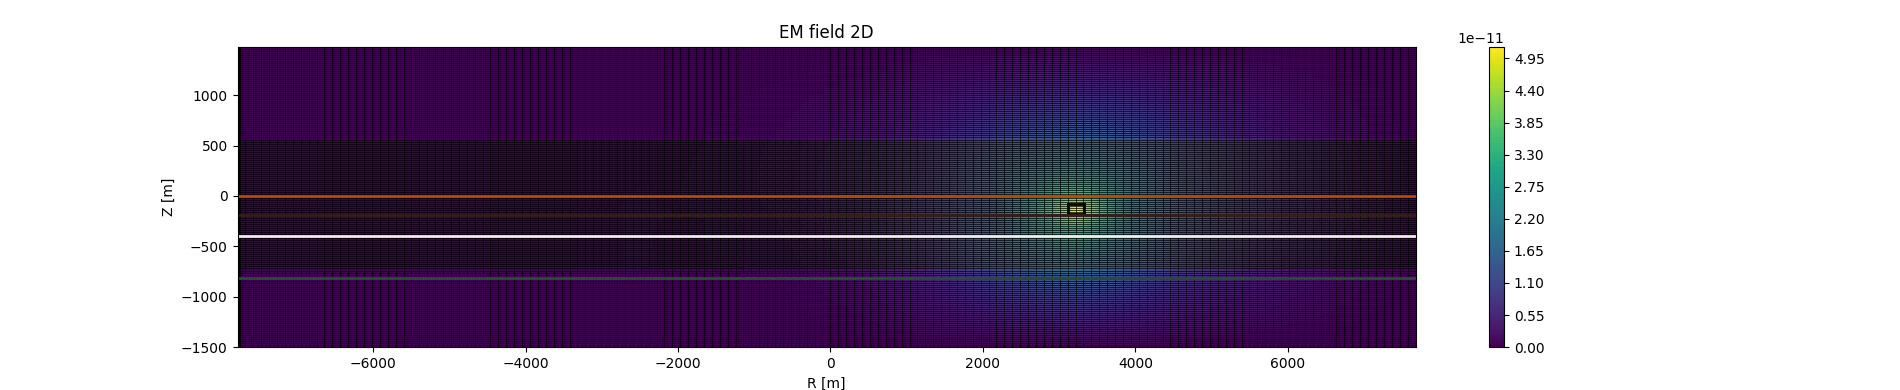
\includegraphics[width=1.0\linewidth]{images/Answer_E_plus_time_layer_1.05.png}
	\caption{Решение $\overrightarrow{\textbf{E}}^+$ при $t = 1.05с$}
	\label{fig:E_plus_t2}
\end{figure} 

Рассмотрим для $t = 1.0, t = 1.025, t = 1.05$ значения $\overrightarrow{\textbf{A}}^+$ и $\overrightarrow{\textbf{E}}^+$ на линии, перпендикулярно проходящей к аномальному объекту по оси $y$ при $x = 0.0, z = -130.0$. Получим следующее:

\begin{figure}
	\centering
	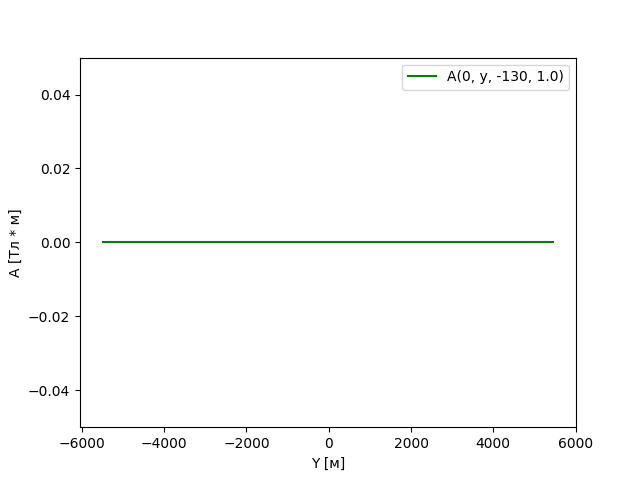
\includegraphics[width=0.5\linewidth]{images/Normal_A(y)_1.png}
	\caption{Решение $\overrightarrow{\textbf{A}}^+$ на линии $(0.0, y, -130.0)$ при $t = 1.0с$}
	\label{fig:A_line_t0}
\end{figure} 

\begin{figure}
	\centering
	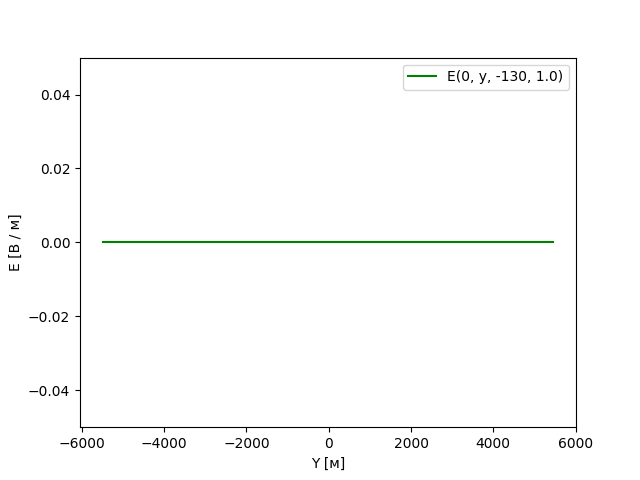
\includegraphics[width=0.5\linewidth]{images/Normal_E(y)_1.png}
	\caption{Решение $\overrightarrow{\textbf{E}}^+$ на линии $(0.0, y, -130.0)$ при $t = 1.0с$}
	\label{fig:E_line_t0}
\end{figure} 

\begin{figure}
	\centering
	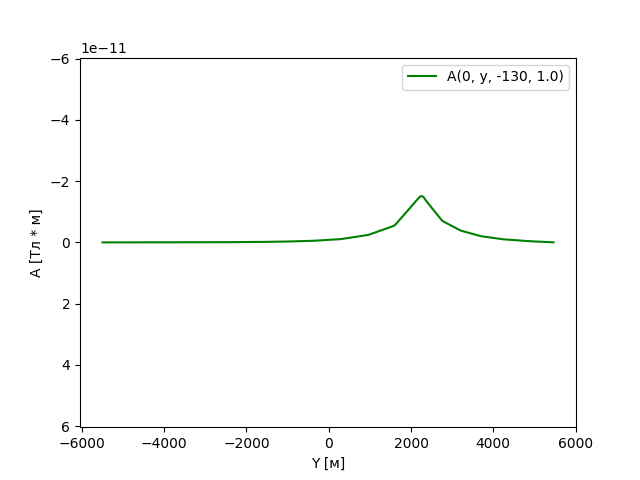
\includegraphics[width=0.5\linewidth]{images/Normal_A(y)_2.png}
	\caption{Решение $\overrightarrow{\textbf{A}}^+$ на линии $(0.0, y, -130.0)$ при $t = 1.025с$}
	\label{fig:A_line_t1}
\end{figure} 

\begin{figure}
	\centering
	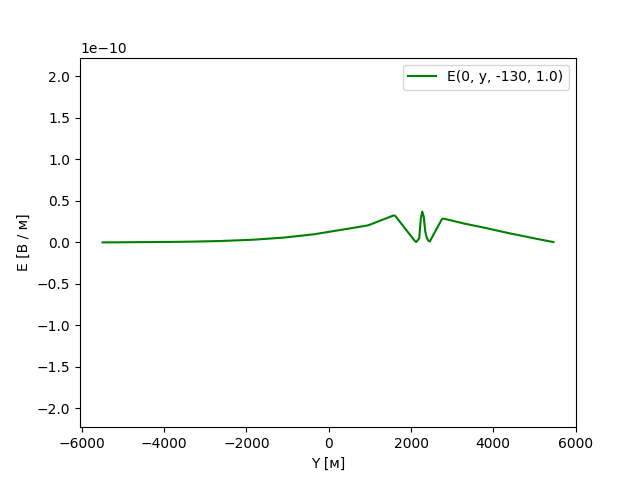
\includegraphics[width=0.5\linewidth]{images/Normal_E(y)_2.png}
	\caption{Решение $\overrightarrow{\textbf{E}}^+$ на линии $(0.0, y, -130.0)$  при $t = 1.025с$}
	\label{fig:E_line_t1}
\end{figure} 

\begin{figure}
	\centering
	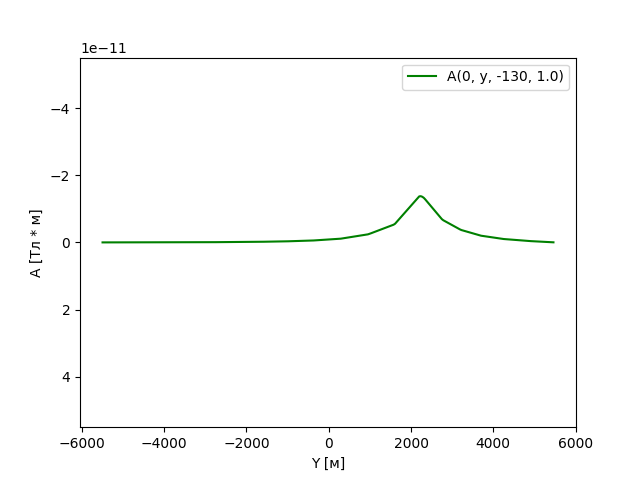
\includegraphics[width=0.5\linewidth]{images/Normal_A(y)_3.png}
	\caption{Решение $\overrightarrow{\textbf{A}}^+$ на линии $(0.0, y, -130.0)$  при $t = 1.05с$}
	\label{fig:A_line_t2}
\end{figure} 

\begin{figure}
	\centering
	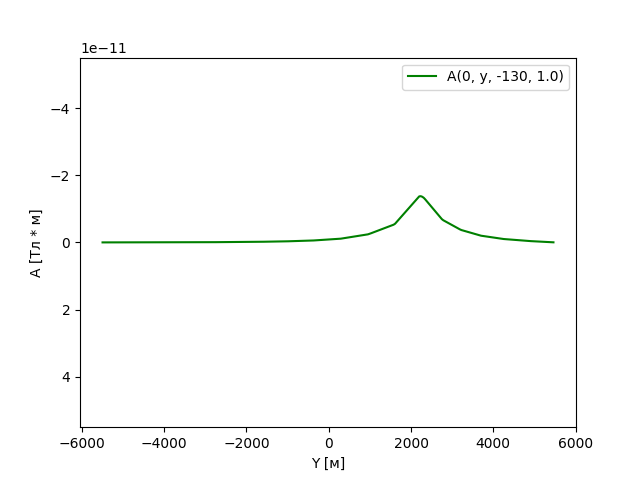
\includegraphics[width=0.5\linewidth]{images/Normal_A(y)_3.png}
	\caption{Решение $\overrightarrow{\textbf{A}}^+$ на линии $(0.0, y, -130.0)$  при $t = 1.05с$}
	\label{fig:E_line_t2}
\end{figure} 


Суммируем полученный результат с нормальным полем и получим состояние поля в разные моменты времени, изображённые на рисунках \ref{fig:A_Istage_t0} -- \ref{fig:E_Istage_t2}.

\begin{figure}
	\centering
	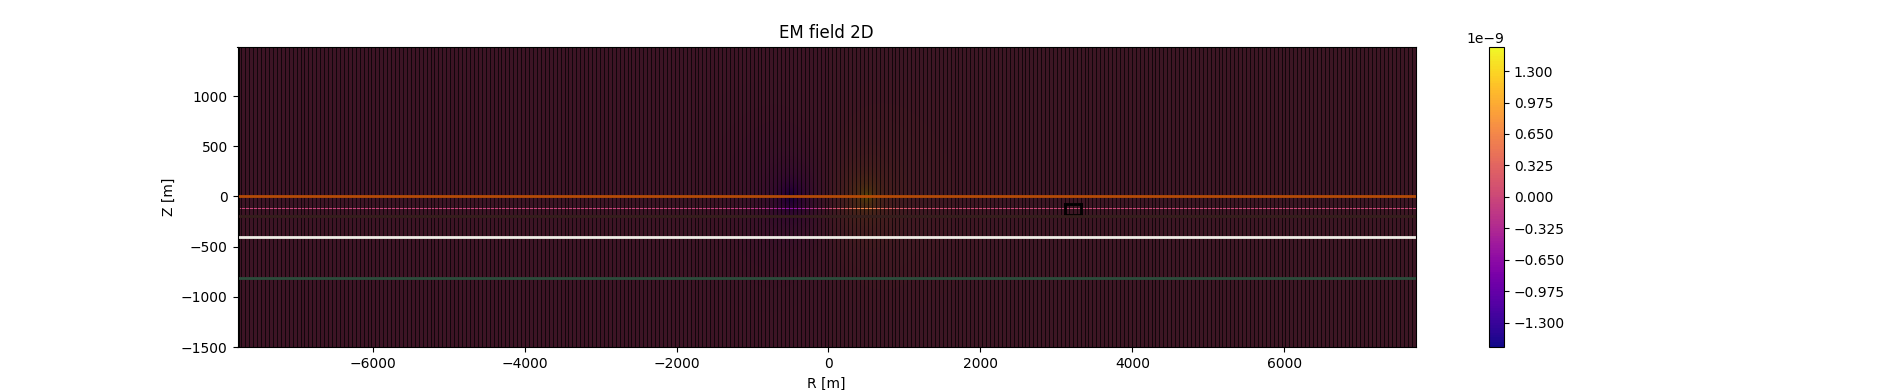
\includegraphics[width=1.0\linewidth]{images/Answer_A_Istage_time_layer_1.png}
	\caption{Решение суммарного поля $\overrightarrow{\textbf{A}}$ при $t = 1.0с$}
	\label{fig:A_Istage_t0}
\end{figure} 


\begin{figure}
	\centering
	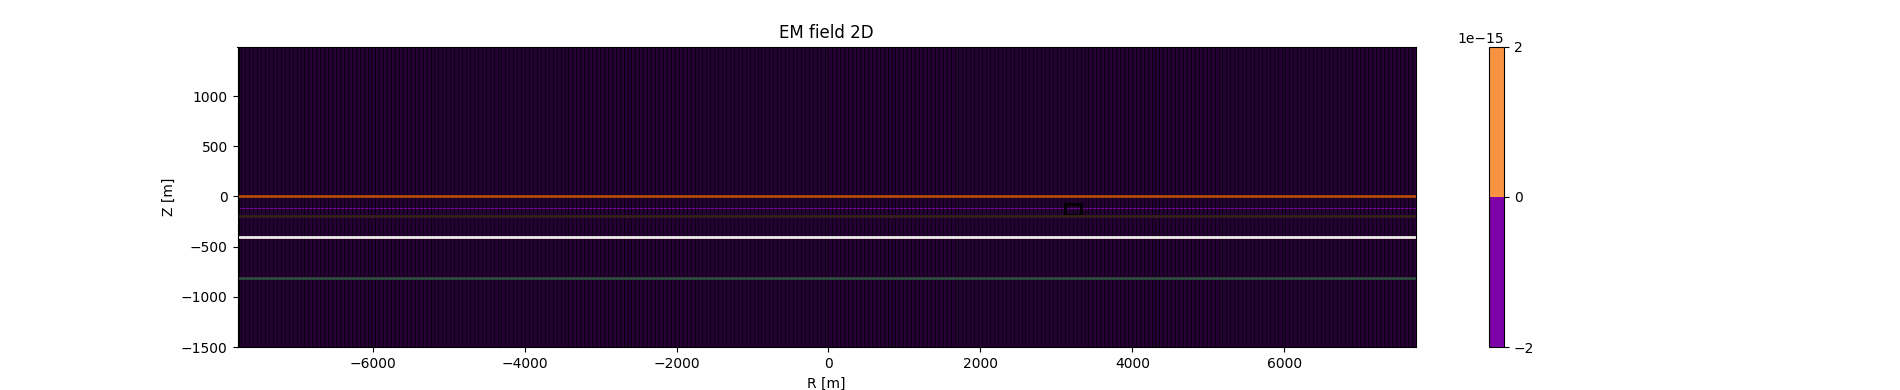
\includegraphics[width=1.0\linewidth]{images/Answer_E_Istage_time_layer_1.png}
	\caption{Решение суммарного поля $\overrightarrow{\textbf{E}}$ при $t = 1.0с$}
	\label{fig:E_Istage_t0}
\end{figure} 


\begin{figure}
	\centering
	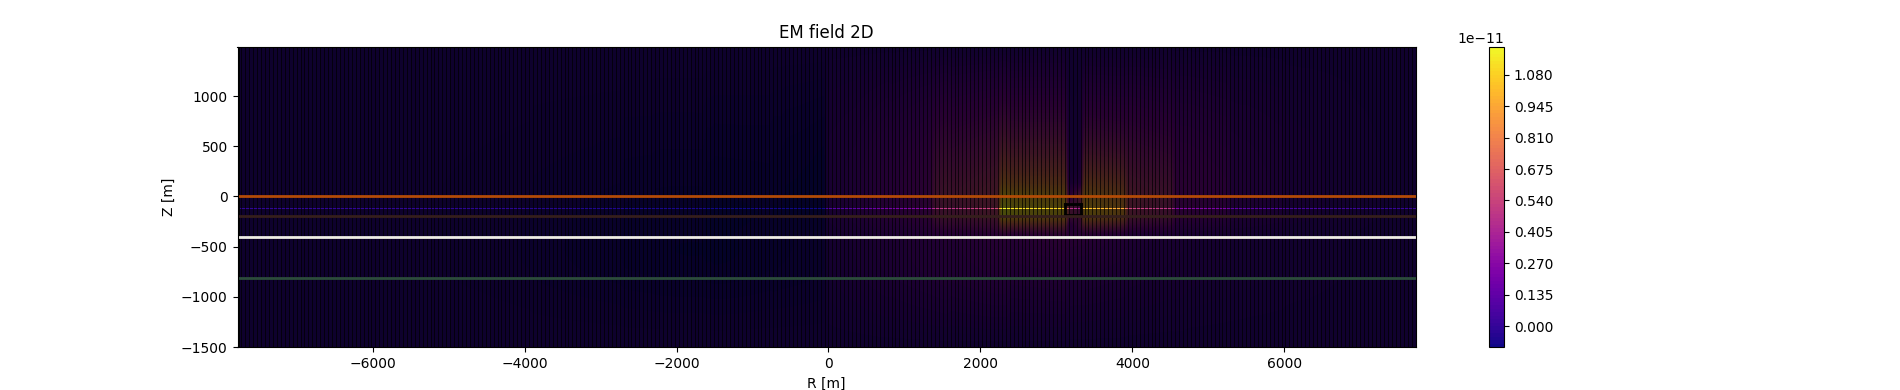
\includegraphics[width=1.0\linewidth]{images/Answer_A_Istage_time_layer_1.0250000000000006.png}
	\caption{Решение суммарного поля $\overrightarrow{\textbf{A}}$ при $t = 1.025с$}
	\label{fig:A_Istage_t1}
\end{figure} 


\begin{figure}
	\centering
	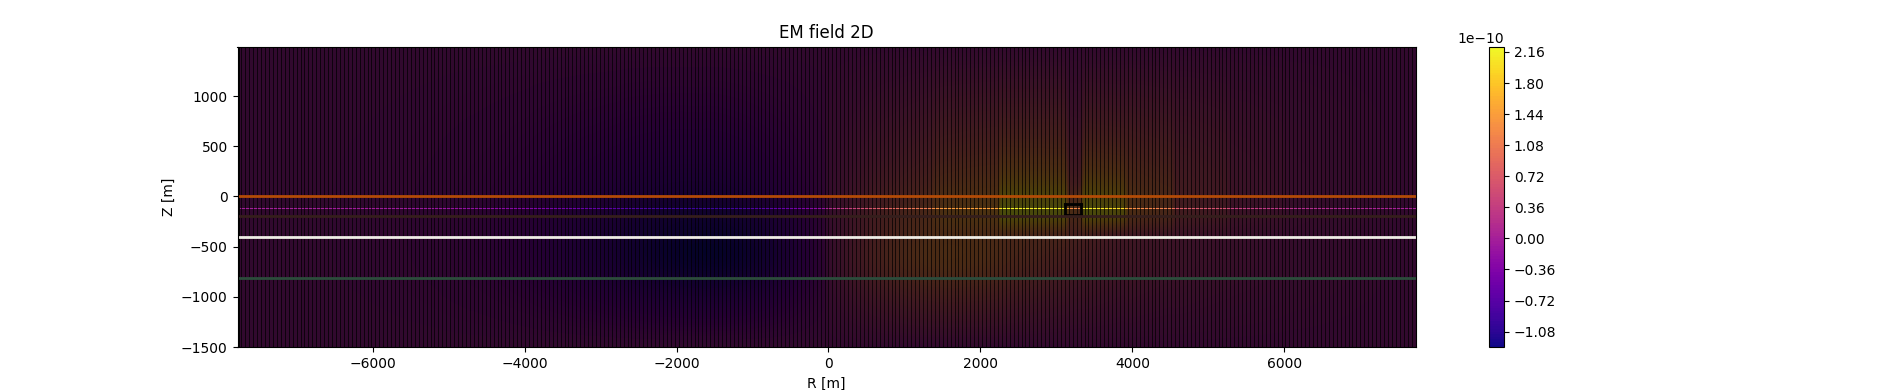
\includegraphics[width=1.0\linewidth]{images/Answer_E_Istage_time_layer_1.0250000000000006.png}
	\caption{Решение суммарного поля $\overrightarrow{\textbf{E}}$ при $t = 1.025с$}
	\label{fig:E_Istage_t1}
\end{figure} 

\begin{figure}
	\centering
	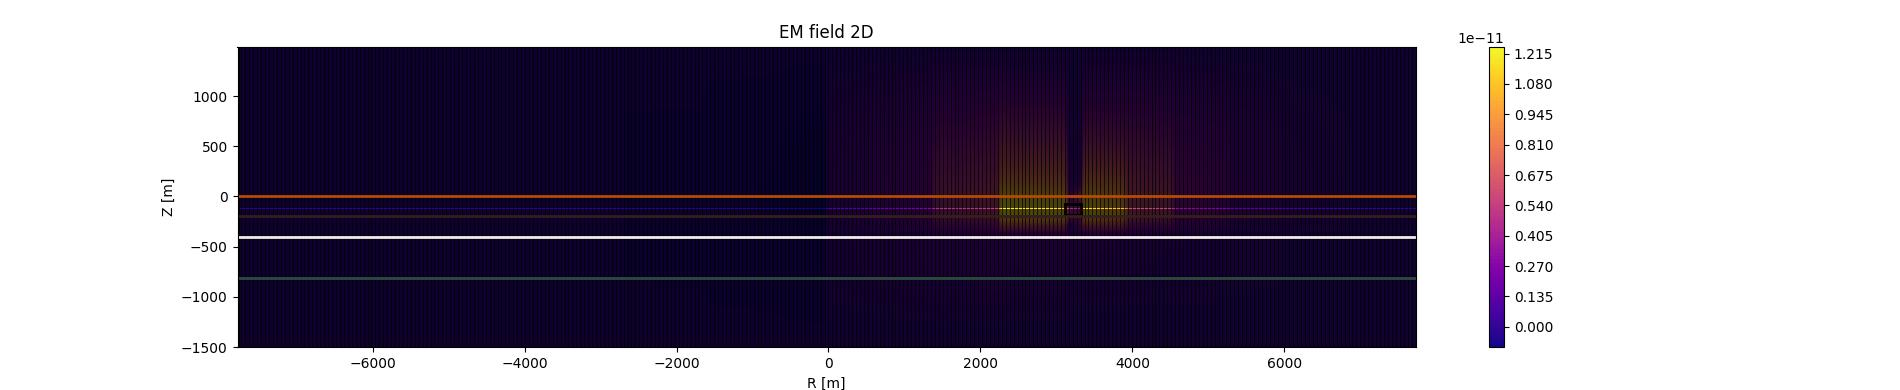
\includegraphics[width=1.0\linewidth]{images/Answer_A_Istage_time_layer_1.05.png}
	\caption{Решение суммарного поля $\overrightarrow{\textbf{A}}$ при $t = 1.05с$}
	\label{fig:A_Istage_t2}
\end{figure} 


\begin{figure}
	\centering
	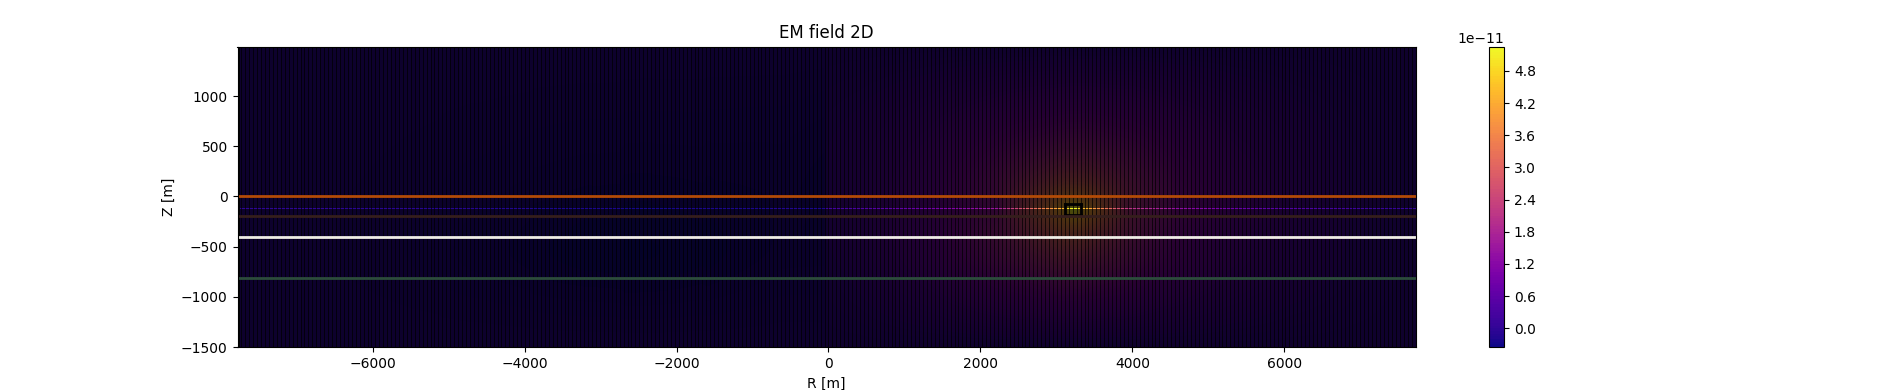
\includegraphics[width=1.0\linewidth]{images/Answer_E_Istage_time_layer_1.05.png}
	\caption{Решение суммарного поля $\overrightarrow{\textbf{E}}$ при $t = 1.05с$}
	\label{fig:E_Istage_t2}
\end{figure} 

Полученные значения \ref{fig:A_Log_added} -- \ref{fig:E_Log_added} $\overrightarrow{\textbf{A}}$ и $\overrightarrow{\textbf{E}}$ рассмотрим на приёмниках.

\begin{figure}
	\centering
	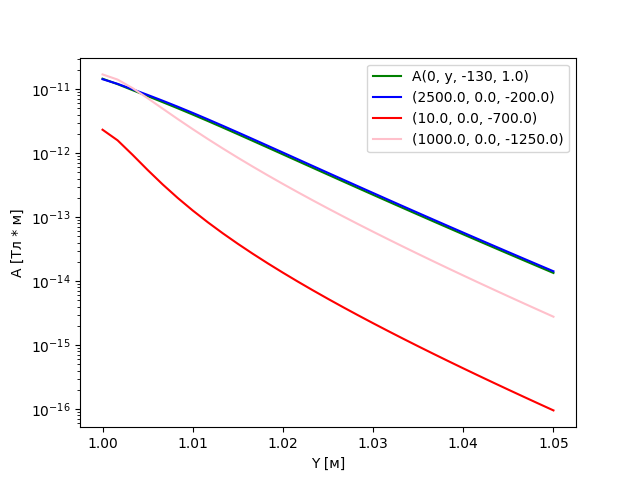
\includegraphics[width=0.8\linewidth]{images/Log_A_obj1.png}
	\caption{Решение суммарного поля $\overrightarrow{\textbf{E}}$ при $t = 1.05с$}
	\label{fig:A_Log_added}
\end{figure} 


\begin{figure}
	\centering
	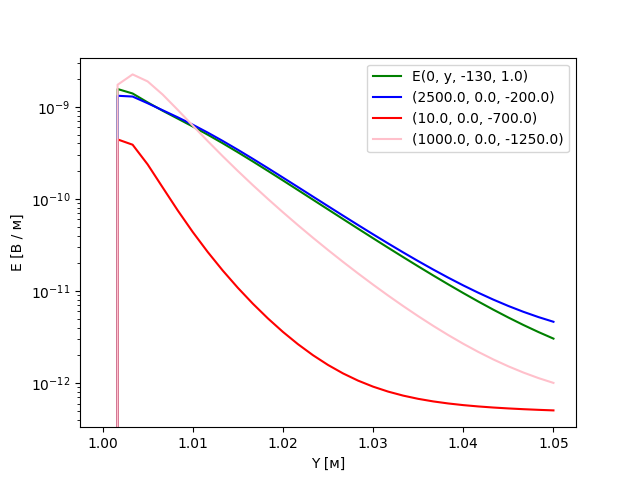
\includegraphics[width=0.8\linewidth]{images/Log_E_obj1.png}
	\caption{Решение суммарного поля $\overrightarrow{\textbf{E}}$ при $t = 1.05с$}
	\label{fig:E_Log_added}
\end{figure} 

Сравнивая показатели на приёмниках до добавления аномалии \ref{fig:LogA} -- \ref{fig:LogE} и после \ref{fig:A_Log_added} -- \ref{fig:A_Log_added}, можно заметить, что значения напряжённости электрического поля на красном приёмнике претерпели наиболее сильные изменения, т.к. он стал более похожим на гиперболу, нежели прямую линию. Значения на синем приёмнике начали изменяться уже в последние сотые секунды исследования. 

\section{Исследование многоэтапного разделения нормального и добавочных полей}

Добавим ещё один аномальный объект со следующими границами: $[-1305; -1050]_x \times [-2255; -2178]_y \times [-1250; -800]_z$ и значением $\sigma = 17$. Будем искать решение из уравнения на добавочное поле (\ref{eq_1_6}). Получим решения в разные моменты времени изображенные на рисунках \ref{fig:A_2plus_t0} -- \ref{fig:E_2plus_t2}.

\begin{figure}
	\centering
	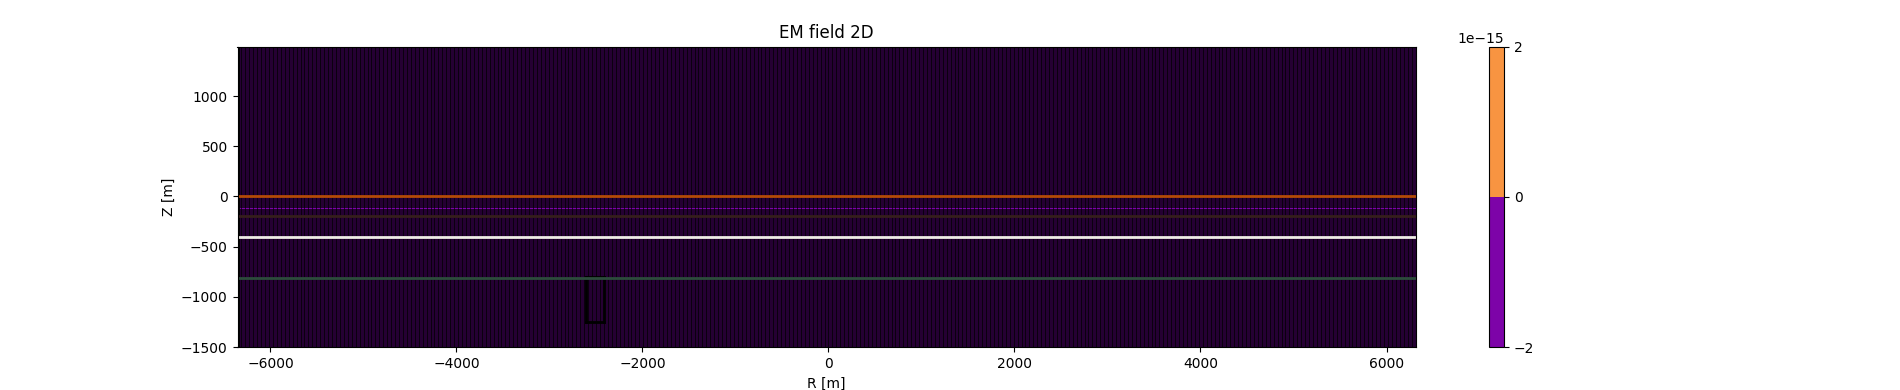
\includegraphics[width=1.0\linewidth]{images/Answer_A_2plus_time_layer_1.png}
	\caption{Решение $\overrightarrow{\textbf{A}}^+$ при $t = 1.0с$}
	\label{fig:A_2plus_t0}
\end{figure} 


\begin{figure}
	\centering
	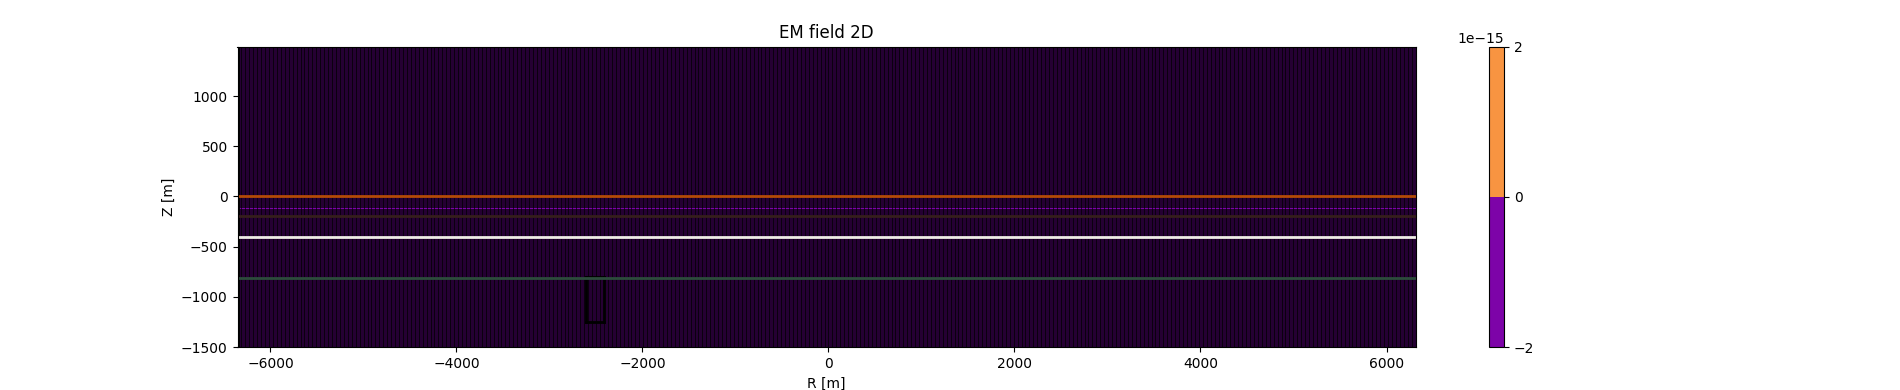
\includegraphics[width=1.0\linewidth]{images/Answer_E_2plus_time_layer_1.png}
	\caption{Решение $\overrightarrow{\textbf{E}}^+$ при $t = 1.0с$}
	\label{fig:E_2plus_t0}
\end{figure} 


\begin{figure}
	\centering
	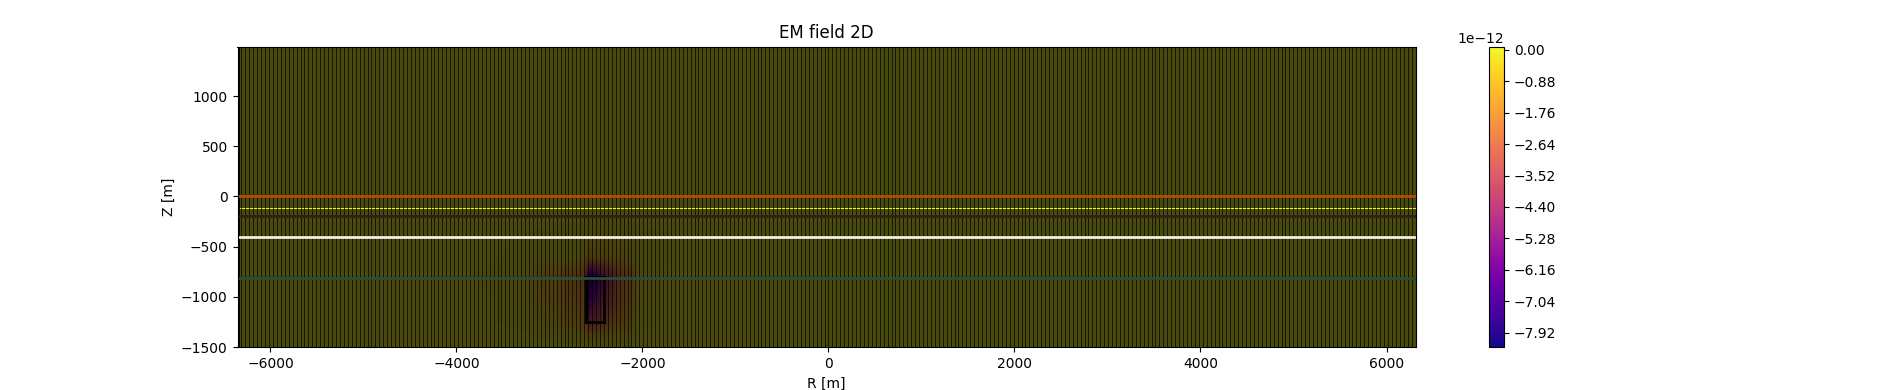
\includegraphics[width=1.0\linewidth]{images/Answer_A_2plus_time_layer_1.0250000000000006.png}
	\caption{Решение $\overrightarrow{\textbf{A}}^+$ при $t = 1.025с$}
	\label{fig:A_2plus_t1}
\end{figure} 


\begin{figure}
	\centering
	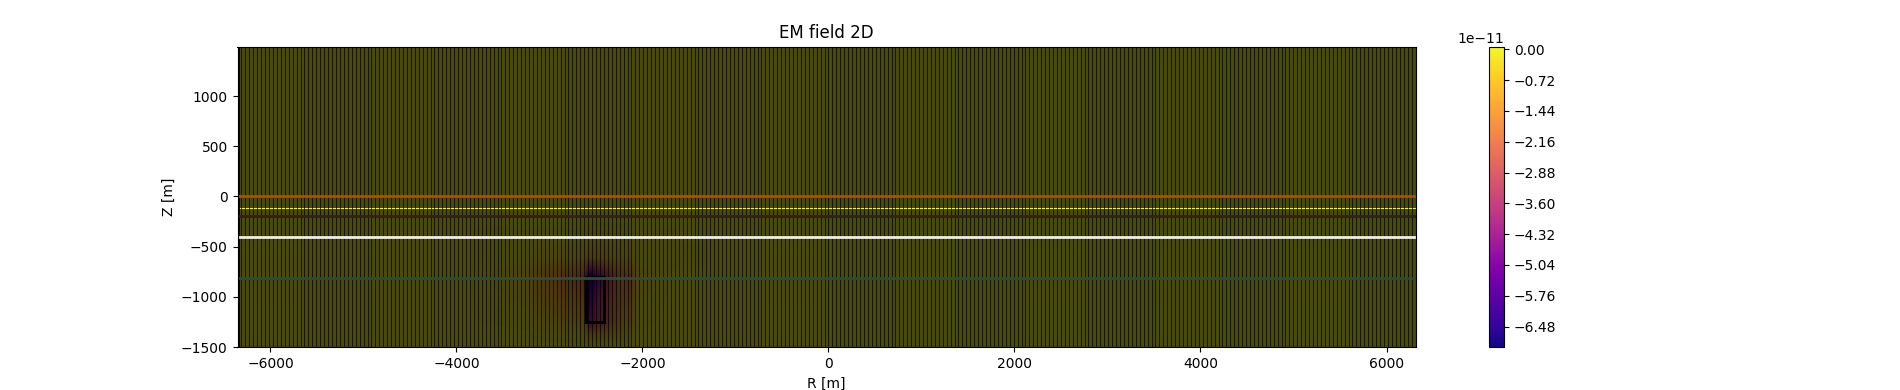
\includegraphics[width=1.0\linewidth]{images/Answer_E_2plus_time_layer_1.0250000000000006.png}
	\caption{Решение $\overrightarrow{\textbf{E}}^+$ при $t = 1.025с$}
	\label{fig:E_2plus_t1}
\end{figure} 

\begin{figure}
	\centering
	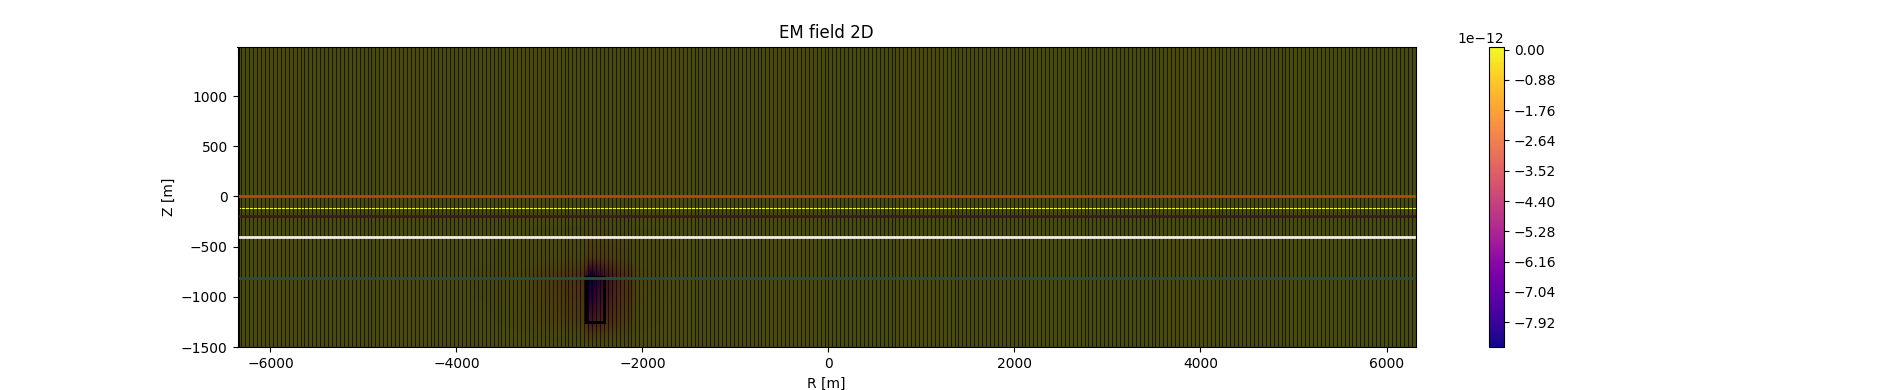
\includegraphics[width=1.0\linewidth]{images/Answer_A_2plus_time_layer_1.05.png}
	\caption{Решение $\overrightarrow{\textbf{A}}^+$ при $t = 1.05с$}
	\label{fig:A_2plus_t2}
\end{figure} 


\begin{figure}
	\centering
	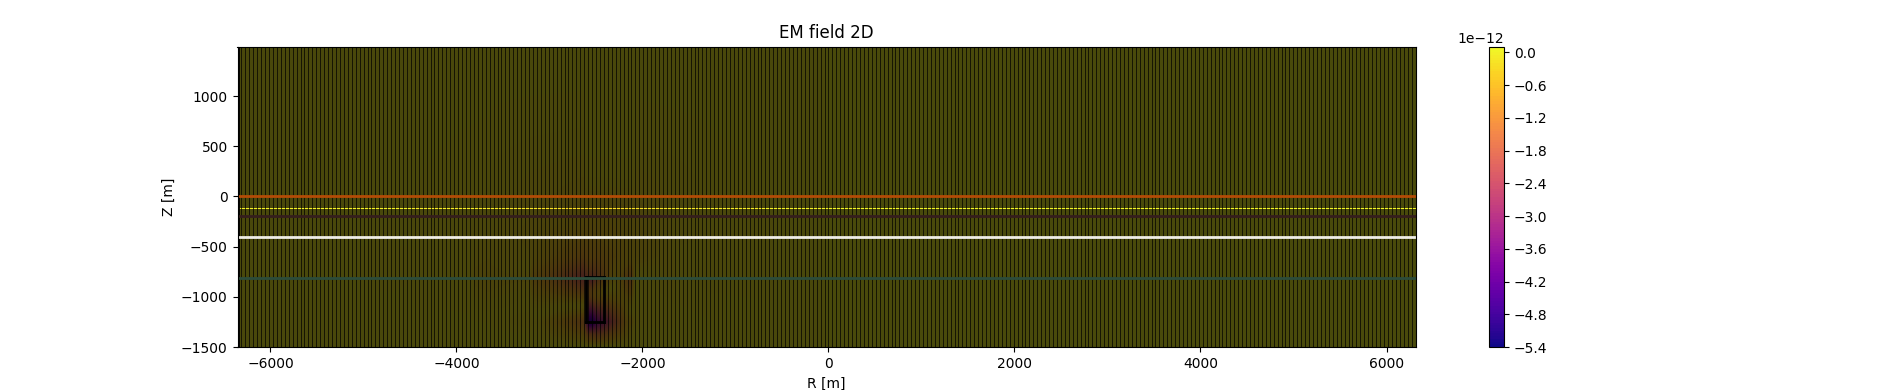
\includegraphics[width=1.0\linewidth]{images/Answer_E_2plus_time_layer_1.05.png}
	\caption{Решение $\overrightarrow{\textbf{E}}^+$ при $t = 1.05с$}
	\label{fig:E_2plus_t2}
\end{figure} 

Рассмотрим для $t = 1.0, t = 1.025, t = 1.05$ значения $\overrightarrow{\textbf{A}}^+$ и $\overrightarrow{\textbf{E}}^+$ на линии, перпендикулярно проходящей к аномальному объекту по оси $y$ при $x = -1177.5, z = -1050.0$. Получим следующее:

\begin{figure}
	\centering
	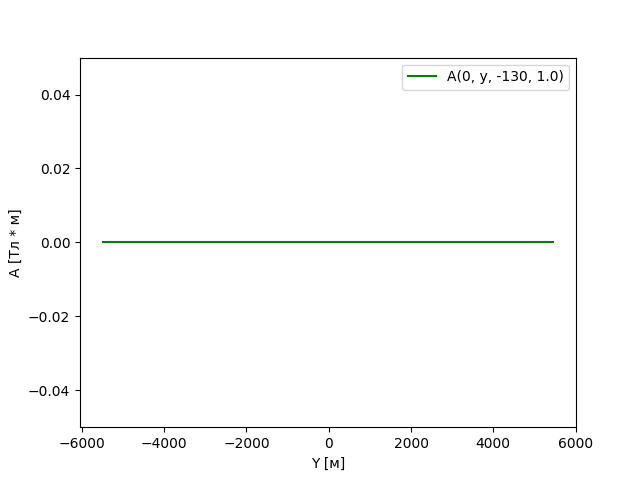
\includegraphics[width=0.5\linewidth]{images/Normal_A_obj2_1.png}
	\caption{Решение $\overrightarrow{\textbf{A}}$ на линии $(0.0, y, -130.0)$ при $t = 1.025с$}
	\label{fig:A_2line_t0}
\end{figure} 

\begin{figure}
	\centering
	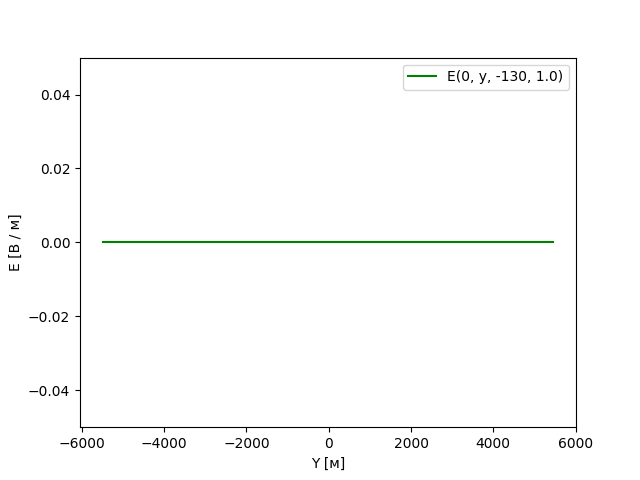
\includegraphics[width=0.5\linewidth]{images/Normal_E_obj2_1.png}
	\caption{Решение $\overrightarrow{\textbf{E}}$ на линии $(0.0, y, -130.0)$ при $t = 1.025с$}
	\label{fig:E_2line_t0}
\end{figure} 

\begin{figure}
	\centering
	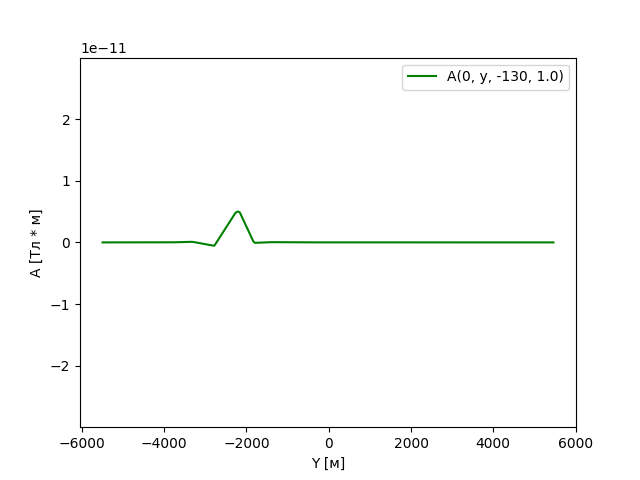
\includegraphics[width=0.5\linewidth]{images/Normal_A_obj2_2.png}
	\caption{Решение $\overrightarrow{\textbf{A}}$ на линии $(0.0, y, -130.0)$ при $t = 1.025с$}
	\label{fig:A_2line_t1}
\end{figure} 

\begin{figure}
	\centering
	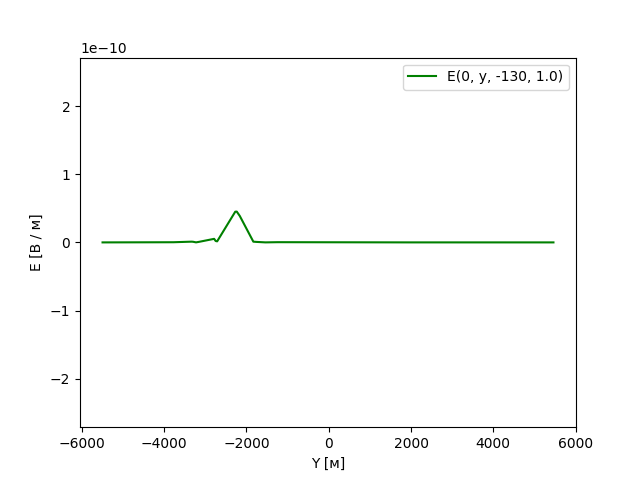
\includegraphics[width=0.5\linewidth]{images/Normal_E_obj2_2.png}
	\caption{Решение $\overrightarrow{\textbf{E}}$ на линии $(0.0, y, -130.0)$  при $t = 1.025с$}
	\label{fig:E_2line_t1}
\end{figure} 

\begin{figure}
	\centering
	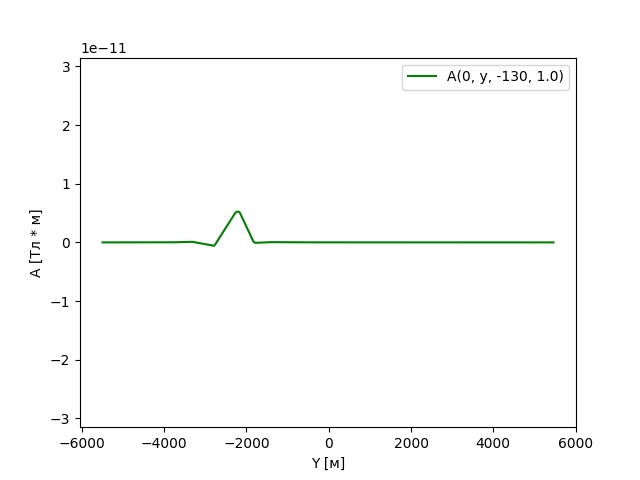
\includegraphics[width=0.5\linewidth]{images/Normal_A_obj2_3.png}
	\caption{Решение $\overrightarrow{\textbf{A}}$ на линии $(0.0, y, -130.0)$  при $t = 1.05с$}
	\label{fig:A_2line_t2}
\end{figure} 

\begin{figure}
	\centering
	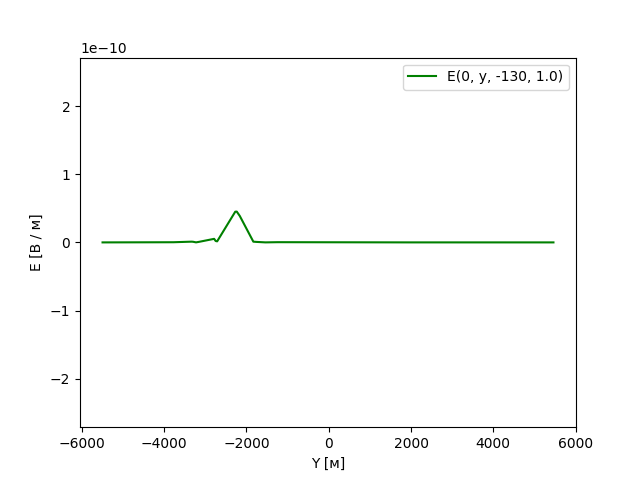
\includegraphics[width=0.5\linewidth]{images/Normal_E_obj2_2.png}
	\caption{Решение $\overrightarrow{\textbf{A}}$ на линии $(0.0, y, -130.0)$  при $t = 1.05с$}
	\label{fig:E_2line_t2}
\end{figure} 

Суммируем полученный результат с полем без аномалий и получим состояние поля в разные моменты времени, изображённые на рисунках \ref{fig:A_IIstage_t0} -- \ref{fig:E_IIstage_t2}.

\begin{figure}
	\centering
	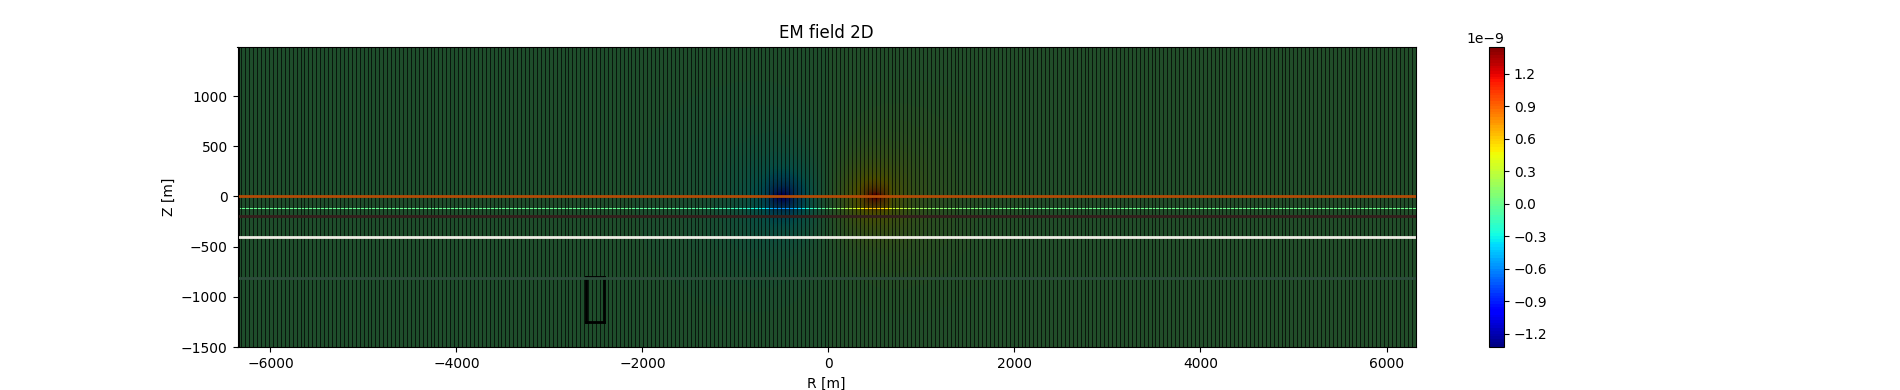
\includegraphics[width=1.0\linewidth]{images/Answer_A_IIstage_time_layer_1.png}
	\caption{Решение суммарного поля $\overrightarrow{\textbf{A}}$ при $t = 1.0с$}
	\label{fig:A_IIstage_t0}
\end{figure} 


\begin{figure}
	\centering
	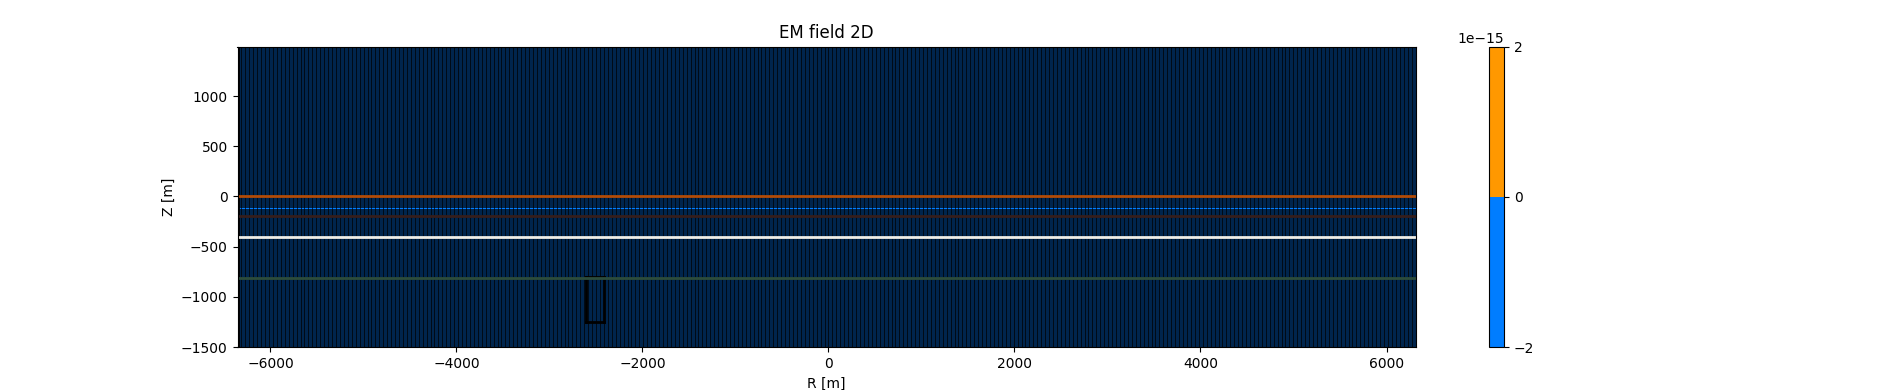
\includegraphics[width=1.0\linewidth]{images/Answer_E_IIstage_time_layer_1.png}
	\caption{Решение суммарного поля $\overrightarrow{\textbf{E}}$ при $t = 1.0с$}
	\label{fig:E_IIstage_t0}
\end{figure} 


\begin{figure}
	\centering
	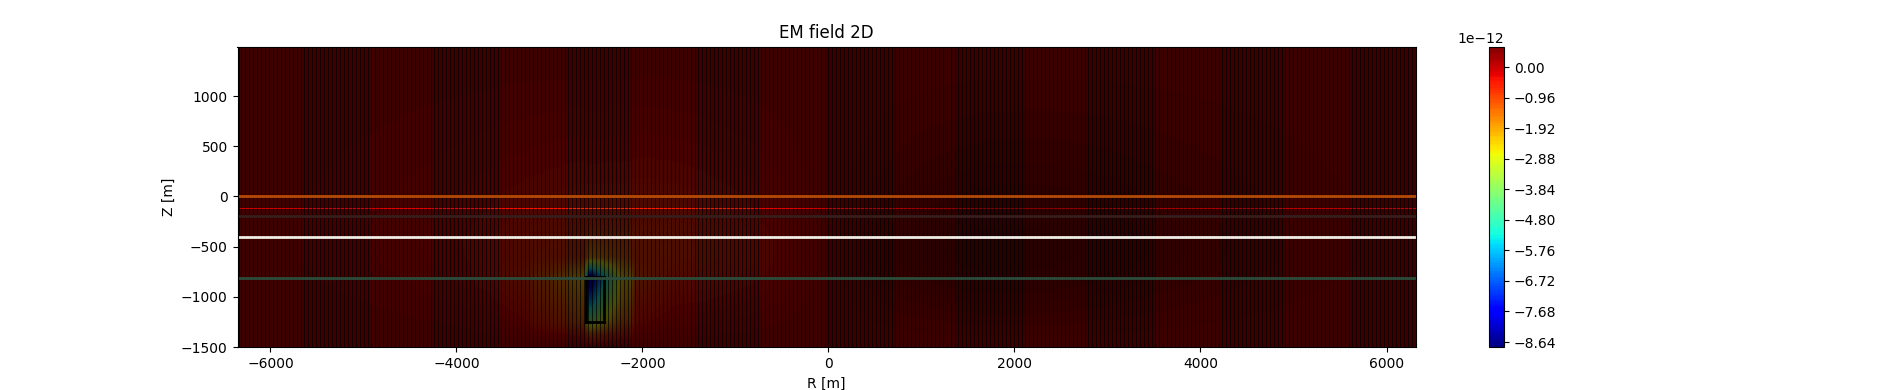
\includegraphics[width=1.0\linewidth]{images/Answer_A_IIstage_time_layer_1.0250000000000006.png}
	\caption{Решение суммарного поля $\overrightarrow{\textbf{A}}$ при $t = 1.025с$}
	\label{fig:A_IIstage_t1}
\end{figure} 


\begin{figure}
	\centering
	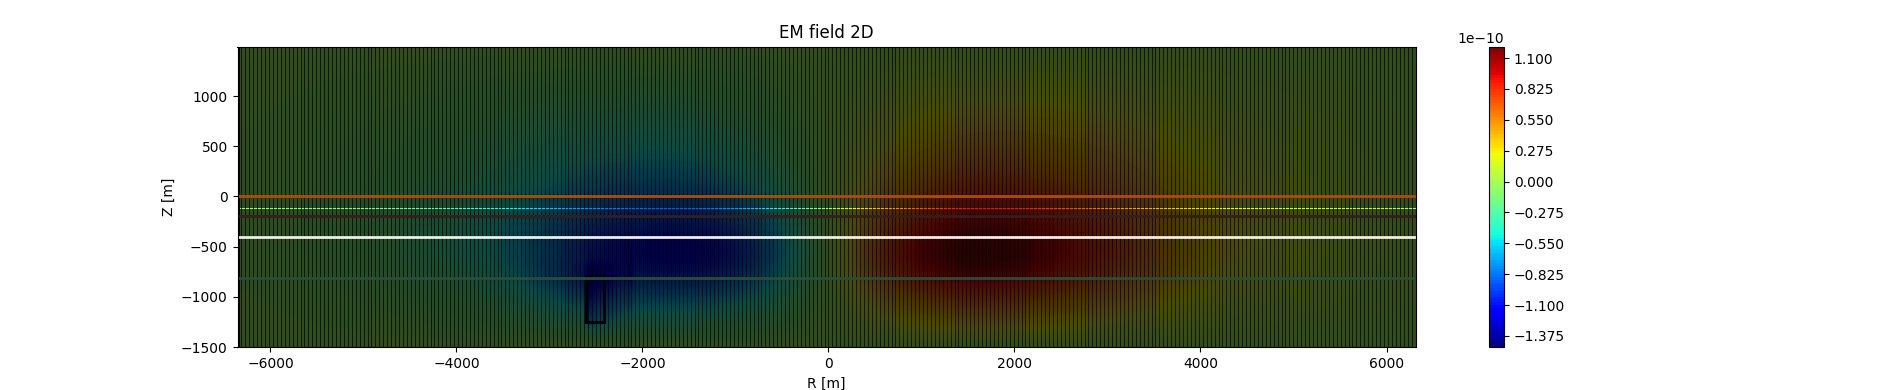
\includegraphics[width=1.0\linewidth]{images/Answer_E_IIstage_time_layer_1.0250000000000006.png}
	\caption{Решение суммарного поля $\overrightarrow{\textbf{E}}$ при $t = 1.025с$}
	\label{fig:E_IIstage_t1}
\end{figure} 

\begin{figure}
	\centering
	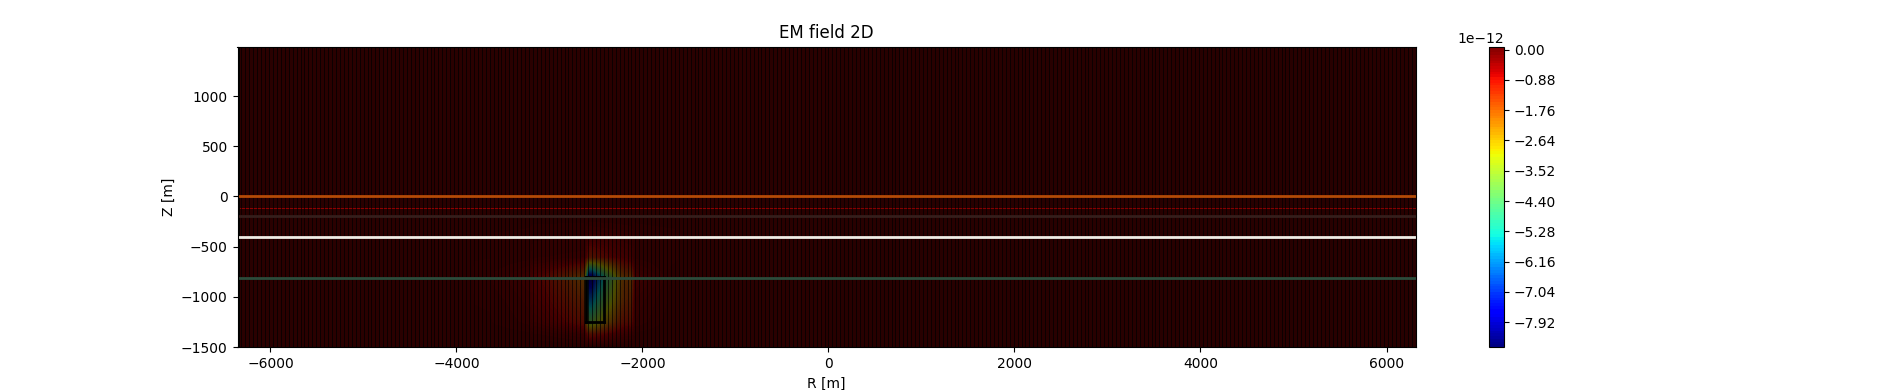
\includegraphics[width=1.0\linewidth]{images/Answer_A_IIstage_time_layer_1.05.png}
	\caption{Решение суммарного поля $\overrightarrow{\textbf{A}}$ при $t = 1.05с$}
	\label{fig:A_IIstage_t2}
\end{figure} 


\begin{figure}
	\centering
	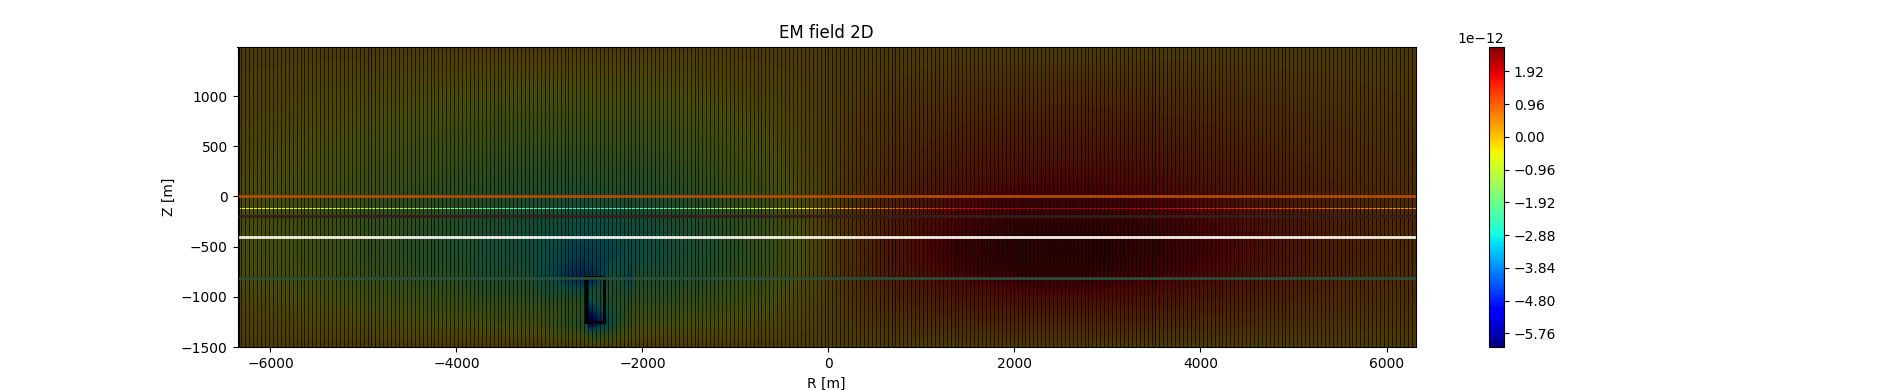
\includegraphics[width=1.0\linewidth]{images/Answer_E_IIstage_time_layer_1.05.png}
	\caption{Решение суммарного поля $\overrightarrow{\textbf{E}}$ при $t = 1.05с$}
	\label{fig:E_IIstage_t2}
\end{figure} 

Полученные значения \ref{fig:A_Log_added2} -- \ref{fig:E_Log_added2} $\overrightarrow{\textbf{A}}$ и $\overrightarrow{\textbf{E}}$ рассмотрим на приёмниках.

\begin{figure}
	\centering
	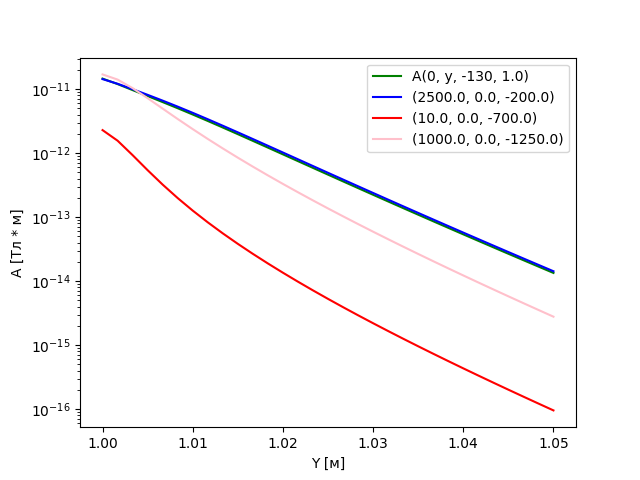
\includegraphics[width=0.8\linewidth]{images/Log_A_obj2.png}
	\caption{Решение суммарного поля $\overrightarrow{\textbf{E}}$ при $t = 1.05с$}
	\label{fig:A_Log_added2}
\end{figure} 


\begin{figure}
	\centering
	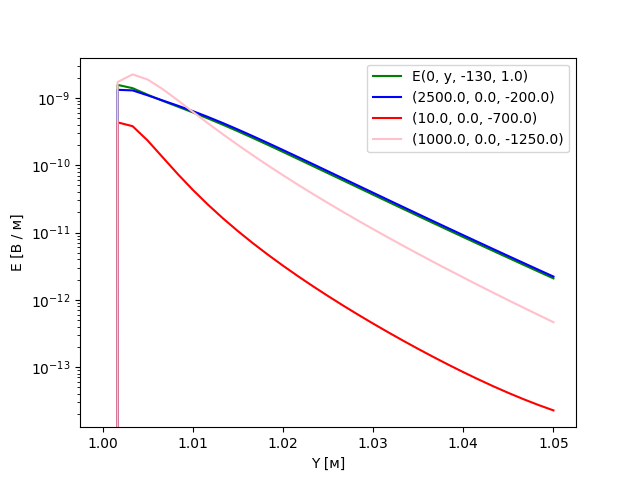
\includegraphics[width=0.8\linewidth]{images/Log_E_obj2.png}
	\caption{Решение суммарного поля $\overrightarrow{\textbf{E}}$ при $t = 1.05с$}
	\label{fig:E_Log_added2}
\end{figure} 

Сравнивая показатели на приёмниках до добавления аномалии \ref{fig:LogA} -- \ref{fig:LogE} и после \ref{fig:A_Log_added2} -- \ref{fig:A_Log_added2}, можно заметить, что значения напряжённости электрического поля ни на одном из приёмников не претерпели изменения, по всей видимости из-за неудачного их расположения. Для изменения ситуации необходимо было бы увеличить размеры расчётной области по пространству и временного диапазона. 

Рассмотрим теперь поле с двумя объектами сразу. Для этого сначала добавим первый объект к чистой расчётной области, после используя его в качестве нормального, добавим вторую аномалию.

\begin{figure}
	\centering
	\includegraphics[width=1.0\linewidth]{images/Answer_A_both_time_layer_1.png}
	\caption{Решение суммарного поля $\overrightarrow{\textbf{A}}$ при $t = 1.0с$}
	\label{fig:A_both_t0}
\end{figure} 


\begin{figure}
	\centering
	\includegraphics[width=1.0\linewidth]{images/Answer_E_both_time_layer_1.png}
	\caption{Решение суммарного поля $\overrightarrow{\textbf{E}}$ при $t = 1.0с$}
	\label{fig:E_both_t0}
\end{figure} 


\begin{figure}
	\centering
	\includegraphics[width=1.0\linewidth]{images/Answer_A_both_time_layer_1.0250000000000006.png}
	\caption{Решение суммарного поля $\overrightarrow{\textbf{A}}$ при $t = 1.025с$}
	\label{fig:A_both_t1}
\end{figure} 


\begin{figure}
	\centering
	\includegraphics[width=1.0\linewidth]{images/Answer_E_both_time_layer_1.0250000000000006.png}
	\caption{Решение суммарного поля $\overrightarrow{\textbf{E}}$ при $t = 1.025с$}
	\label{fig:E_both_t1}
\end{figure} 

\begin{figure}
	\centering
	\includegraphics[width=1.0\linewidth]{images/Answer_A_both_time_layer_1.05.png}
	\caption{Решение суммарного поля $\overrightarrow{\textbf{A}}$ при $t = 1.05с$}
	\label{fig:A_both_t2}
\end{figure} 


\begin{figure}
	\centering
	\includegraphics[width=1.0\linewidth]{images/Answer_E_both_time_layer_1.05.png}
	\caption{Решение суммарного поля $\overrightarrow{\textbf{E}}$ при $t = 1.05с$}
	\label{fig:E_both_t2}
\end{figure} 

Полученные значения \ref{fig:A_Log_both} -- \ref{fig:E_Log_both} $\overrightarrow{\textbf{A}}$ и $\overrightarrow{\textbf{E}}$ рассмотрим на приёмниках.

\begin{figure}
	\centering
	\includegraphics[width=0.8\linewidth]{images/Log_A_both.png}
	\caption{Решение суммарного поля $\overrightarrow{\textbf{E}}$ при $t = 1.05с$}
	\label{fig:A_Log_both}
\end{figure} 


\begin{figure}
	\centering
	\includegraphics[width=0.8\linewidth]{images/Log_E_both.png}
	\caption{Решение суммарного поля $\overrightarrow{\textbf{E}}$ при $t = 1.05с$}
	\label{fig:E_Log_both}
\end{figure} 

Сравнивая показатели на приёмниках до добавления обеих аномалий \ref{fig:LogA} -- \ref{fig:LogE} и после \ref{fig:A_Log_both} -- \ref{fig:E_Log_both}, можно заметить, что значения напряжённости электрического поля на красном приёмнике все те же изменения, что и без учёта второго объекта. Это связано со слабым влиянием второго объекта на приёмники. 